\minitoc

\vfill

In Chapters~\ref{chap::semantic_evaluation} and~\ref{chap::learned_evaluation}, we proposed a semantic quality evaluation of \gls{acr::3d} building models employing a learning formulation.
Herein, we put our pipeline to the test.
First, in Section~\ref{sec::experiments::datasets}, we delineate how the building models that are used for the study are obtained.
Second, Section~\ref{sec::experiments::baseline_feature_analysis} provides a first experimental outlook of the capacity of our approach to detect errors affecting \gls{acr::3d} building models.
Third, in Section~\ref{sec::experiments::scalability}, we study the scalability of the proposed approach under different scenarii.
Finally, in Section~\ref{sec::experiments::finesse}, we analyse results of the experiments at low \textbf{\gls{acr::efin}} levels.

\clearpage

\section{Datasets}
    \label{sec::experiments::datasets}
    In this section, we present the studied building models.
    Section~\ref{subsec::experiments::datasets::scenes} describes the selected urban scenes as well as the modeling technique which helped produce the studied models.
    Next, in Section~\ref{subsec::experiments::datasets::stats}, we analyse the distribution of the previously defined errors (cf. Chapter~\ref{chap::semantic_evaluation}) over the three urban areas of interest.
    
    \subsection{Urban scenes and modeling techniques}
        \label{subsec::experiments::datasets::scenes}        
        \gls{acr::3d} models from three different cities of France are selected in order to assess the performance of our framework: \textbf{Elancourt}, \textbf{Nantes}, and the XIII\textsuperscript{th} district of Paris (\textbf{Paris-13}) (cf. Figure~\ref{fig::france_map}).
        Figure~\ref{fig::elancourt_ortho} depicts the small city of \textbf{Elancourt} which contains diverse types of buildings: residential areas with gable and hip roof buildings and districs with large industrial flat roof buildings (cf. Figure~\ref{subfig::elancourt_samples}).
        \textbf{Nantes}, as shown in Figure~\ref{fig::nantes_ortho}, represents a denser urban setting but with a lower building diversity (cf. Figure~\ref{subfig::nantes_samples}).
        In Figure~\ref{fig::paris-13_ortho}, one can see how \textbf{Paris-13} consists of mostly flat roof high towers which coexist with Haussmann style buildings that typically exhibit highly fragmented roofs (cf. Figure~\ref{subfig::paris-13_samples}).
        The \textbf{Elancourt} (\textit{resp.} \textbf{Nantes} and \textbf{Paris-13}) scene contains \num{2009} (\textit{resp.} \num{748} and \num{478}) annotated building models.
        In order to handle these models, \verb!proj.city!\footnote{
            \verb!proj.city!: \href{https://github.com/ethiy/proj.city}{\url{https://github.com/ethiy/proj.city}}
        }, a \verb!C++! library, was developed making use of the \verb!CGAL! library~\parencite{fabri2000design}.
        Thanks to this tool, we can project building models in the nadir direction as well as produce the corresponding height maps.
        The \gls{acr::dsm} and the orthorectified image spatial resolution is \SI{0.06}{\m} for the first area while it is \SI{0.1}{\m} for the other ones.\\

        \begin{figure}[htb]
            \ffigbox[\textwidth]{
                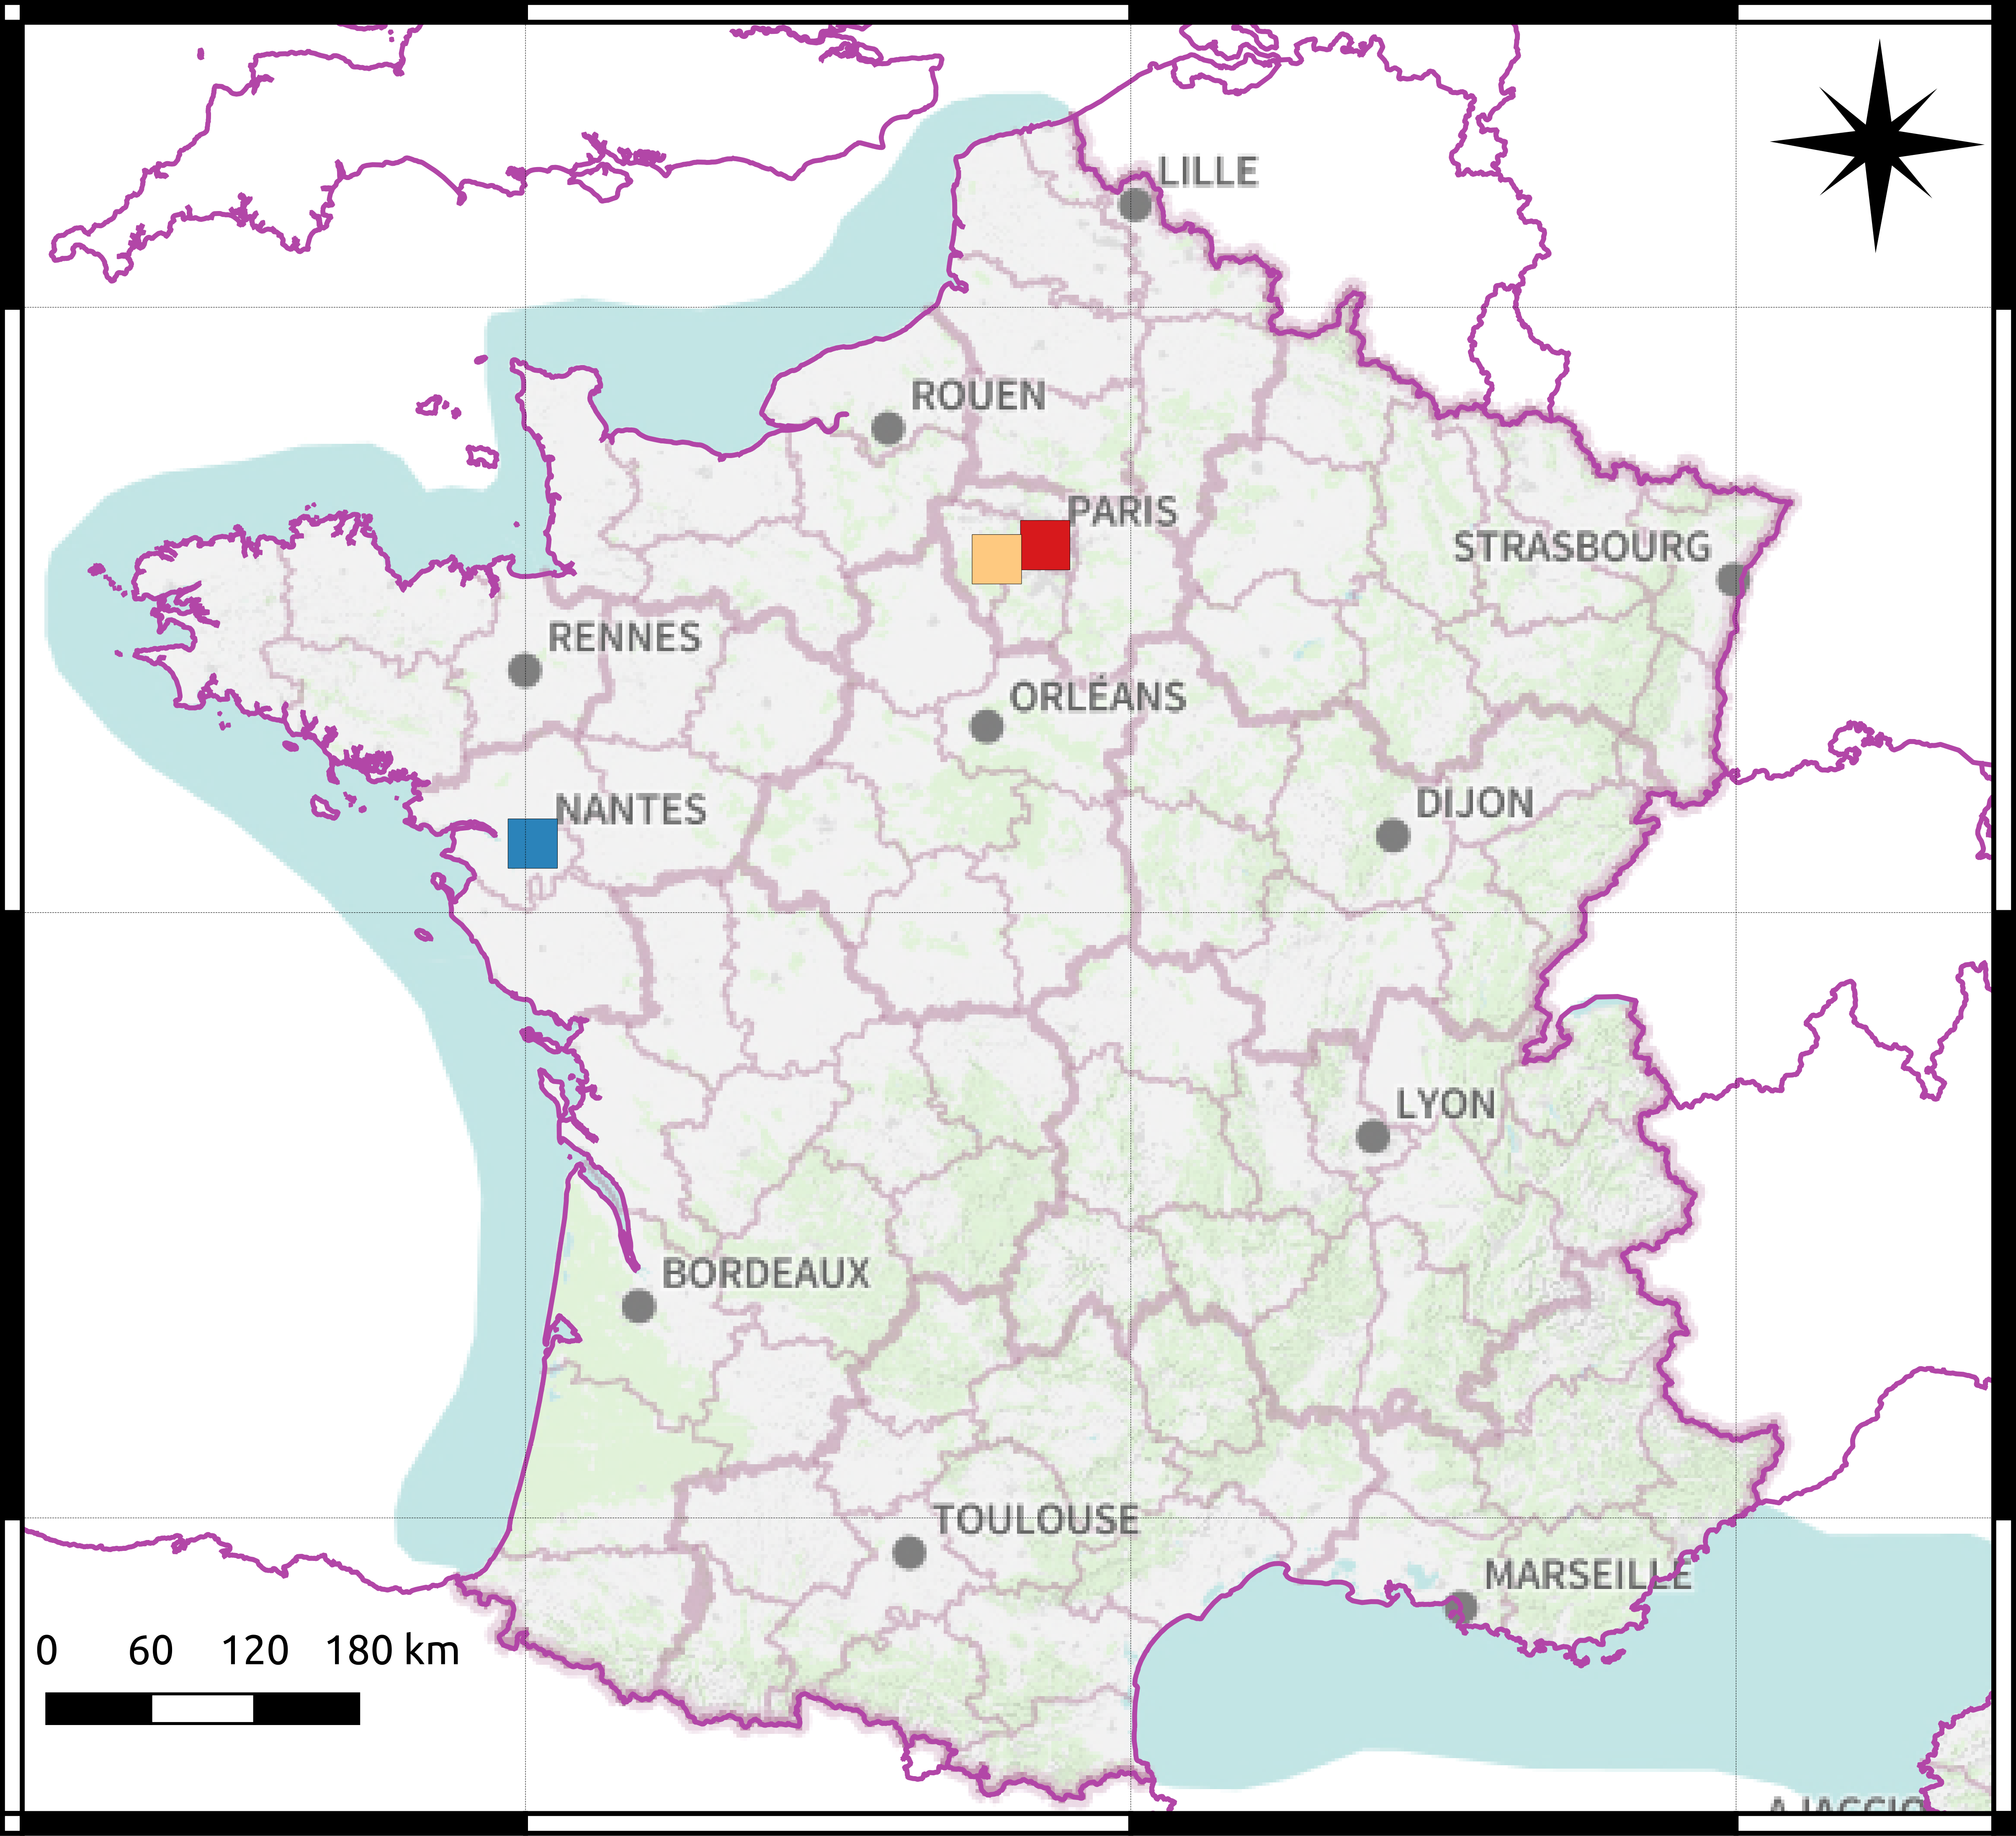
\includegraphics[width=.75\textwidth]{images/datasets/france_map}
            }{
                \caption[
                    Map of France showing the studied urban scenes.
                ]{
                    \label{fig::france_map}
                    Map of France showing the studied urban scenes.
                    Each square corresponds to a city:
                    \textcolor[rgb]{.84,.1,.11}{\(\blacksquare\)} \textbf{Paris-13}, \textcolor[rgb]{1,.79,.5}{\(\blacksquare\)} \textbf{Elancourt}, \textcolor[rgb]{.17,.51,.73}{\(\blacksquare\)} \textbf{Nantes}.
                }
            }
        \end{figure}

        \begin{figure}[htb]
            \ffigbox[\FBwidth]{
                \includegraphics[width=\textwidth]{images/datasets/elancourt_global}
            }{
                \caption{
                    \label{fig::elancourt_ortho}
                    Orthoimage showing the diversity of buildings in Elancourt.
                }
            }
        \end{figure}

        \begin{figure}[htb]
            \ffigbox[\FBwidth]{
                \includegraphics[width=\textwidth]{images/datasets/nantes_global}
            }{
                \caption{
                    \label{fig::nantes_ortho}
                    Orthoimage depicting the dense city center of Nantes.
                }
            }
        \end{figure}

        \begin{figure}[htb]
            \ffigbox[\FBwidth]{
                \includegraphics[width=\textwidth]{images/datasets/paris-13_global}
            }{
                \caption{
                    \label{fig::paris-13_ortho}
                    Orthoimage showing the heterogeneity of the XIII\textsuperscript{th} district of Paris.
                }
            }
        \end{figure}

        \begin{figure}[htb]
            \ffigbox[\textwidth]{
                \begin{subfloatrow}[3]
                    \ffigbox[\FBwidth]{
                        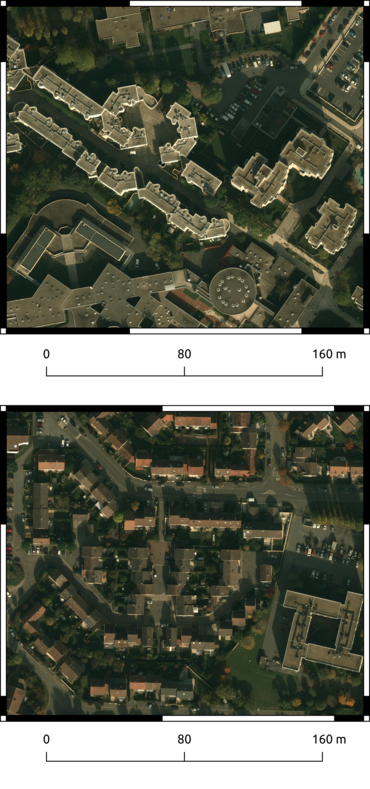
\includegraphics[width=.3\textwidth]{images/datasets/elancourt_samples}
                    }{
                        \caption{
                            \label{subfig::elancourt_samples}
                            Elancourt contains flat roof buildings (top) as well as gable roof ones (bottom).
                        }
                    }
                    \ffigbox[\FBwidth]{
                        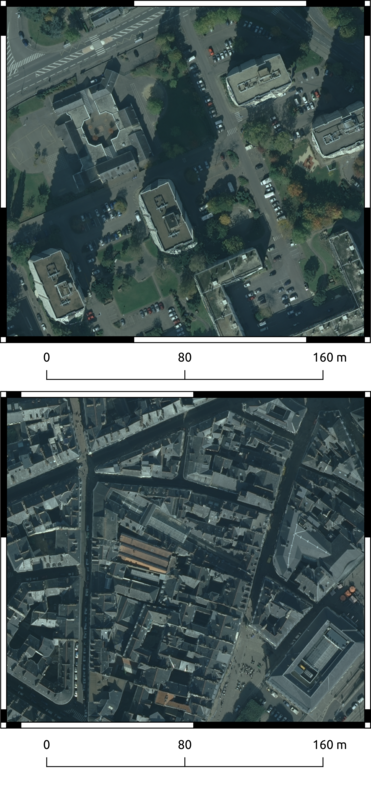
\includegraphics[width=.3\textwidth]{images/datasets/nantes_samples}
                    }{
                        \caption{
                            \label{subfig::nantes_samples}
                            Nantes exhibits high rising towers (top) along densely packed fragmented roof buildings (bottom).
                        }
                    }
                    \ffigbox[\FBwidth]{
                        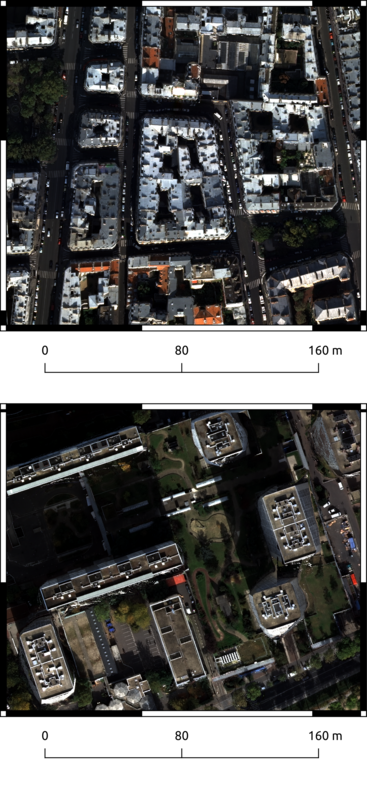
\includegraphics[width=.3\textwidth]{images/datasets/paris-13_samples}
                    }{
                        \caption{
                            \label{subfig::paris-13_samples}
                            The XIII\textsuperscript{th} district of Paris is made of Haussmannian buildings (top) and high rising towers bottom).
                        }
                    }
                \end{subfloatrow}
            }{
                \caption{
                    \label{fig::samples}
                    Samples of building types per area of interest.
                }
            }
        \end{figure}

        Bati3D\textsuperscript{\textregistered} models were used in these experiments (cf. Figure~\ref{fig::method_modeling}).
        This product is based on the algorithm described in~\parencite{durupt2006automatic}.
        The latter generates models  out of existing building footprints and aerial \gls{acr::vhr} multi-view \glspl{acr::dsm}.
        The modeling algorithm simulates possible roof structures with facets satisfying some geometric constraints.
        The best configuration is selected using a scoring system on the extrapolated roofs.
        Finally, vertical building fa\c{c}ades connect the optimal roof to the building footprint.
        These models have a \gls{acr::lod}-2 level.
        This method has been adapted to roof types of low complexity and favors symmetrical models that are common in residential areas.
        It has been selected to ensure a varying error rate for the three areas of interest, especially since models were generated with partly erroneous cadastral maps.
        Consequently, the modeling will fail, allowing to tackle the evaluation of the ensuing models.
        \num{3235} buildings in total are considered.
        They were annotated according to the atomic errors list provided by our taxonomy.

        \begin{figure}[htb]
            \centering
            \ffigbox[\textwidth]{
                \begin{subfloatrow}[2]
                    \centering
                    \ffigbox[.5\textwidth]{
                        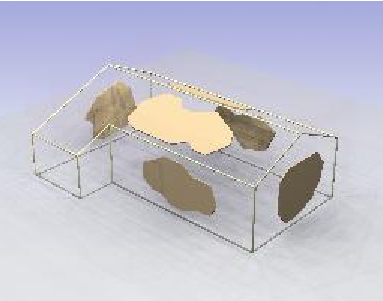
\includegraphics[width=.35\textwidth]{images/bati3d/plane_detection}
                    }{
                        \caption{
                            \label{subfig::plane_detection}
                            Plane extraction.
                        }
                    }
                    \ffigbox[.5\textwidth]{
                        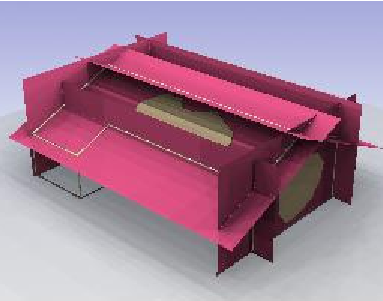
\includegraphics[width=.35\textwidth]{images/bati3d/plane_arrangements}
                    }{
                        \caption{
                            \label{subfig::arrangements}
                            Plane arrangement building.
                        }
                    }
                \end{subfloatrow}
                \vskip1em
                \begin{subfloatrow}[2]
                    \centering
                    \ffigbox[.5\textwidth]{
                        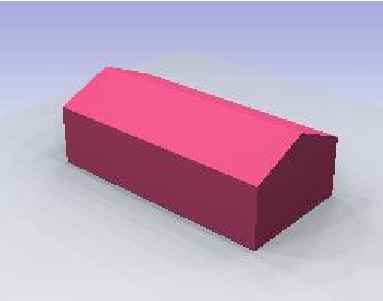
\includegraphics[width=.35\textwidth]{images/bati3d/bati3d}
                    }{
                        \caption{
                            \label{subfig::bati3d}
                            Estimating the building structure.
                        }
                    }
                    \ffigbox[.5\textwidth]{
                        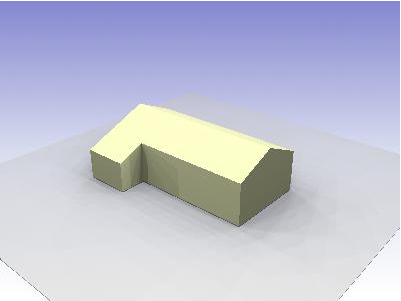
\includegraphics[width=.35\textwidth]{images/bati3d/reel}
                    }{
                        \caption{
                            \label{subfig::reel}
                            The ground truth model.
                        }
                    }
                \end{subfloatrow}
            }{
                \caption[
                    Illustration of how the modeling steps of the approach presented in~\parencite{durupt2006automatic}.
                ]{
                    \label{fig::method_modeling}
                    Illustration of how the modeling steps of the approach presented in~\parencite{durupt2006automatic}.
                    A first step consists of plane extraction (cf. Figure~\ref{subfig::plane_detection}).
                    Out the resulting plane arrangements (cf. Figure~\ref{subfig::arrangements}), the most plausible building structure is chosen (cf. Figure~\ref{subfig::bati3d}).
                    Figure~\ref{subfig::reel} shows the ground truth model.
                    Images taken from~\parencite{bredif20103d}.
                }
            }
        \end{figure}

    \subsection{Error statistics}
        \label{subsec::experiments::datasets::stats}
        Each one of these scenes contains more than \num{10000} buildings each.
        Only a small fraction of these building models were annotated in the aim of building a training dataset.
        To annotate a building model, the manual operator compares the nadir projection of the model to the corresponding orthoimage and \gls{acr::dsm}.
        This was possible thanks to the work\footnote{\verb!sGrISner!: \href{https://github.com/CHUPClem/sGrISner}{\url{https://github.com/sGrISner/sGrISner}}} of Clémence Chupin, who was a Master student at \gls{acr::ensg}.
        She helped develop a \verb!pyQT! interface in order to ease the task.
        This allows to switch between data sources and better assess the errors\footnote{There can be multiple errors per building.} affecting each building.
        This tool can also be used in the case of active learning where the operator validates or corrects the predictions from a classifier which is connected in the backend.
        Figure~\ref{fig::annotation_tool} shows how the \verb!sGrISner! interface enables the operator to compare the building model to the orthoimage in order to assign the correct labels.\\

        \begin{figure}[htb]
            \centering
            \ffigbox[\textwidth]{
                \begin{subfloatrow}
                    \centering
                    \ffigbox[\textwidth]{
                        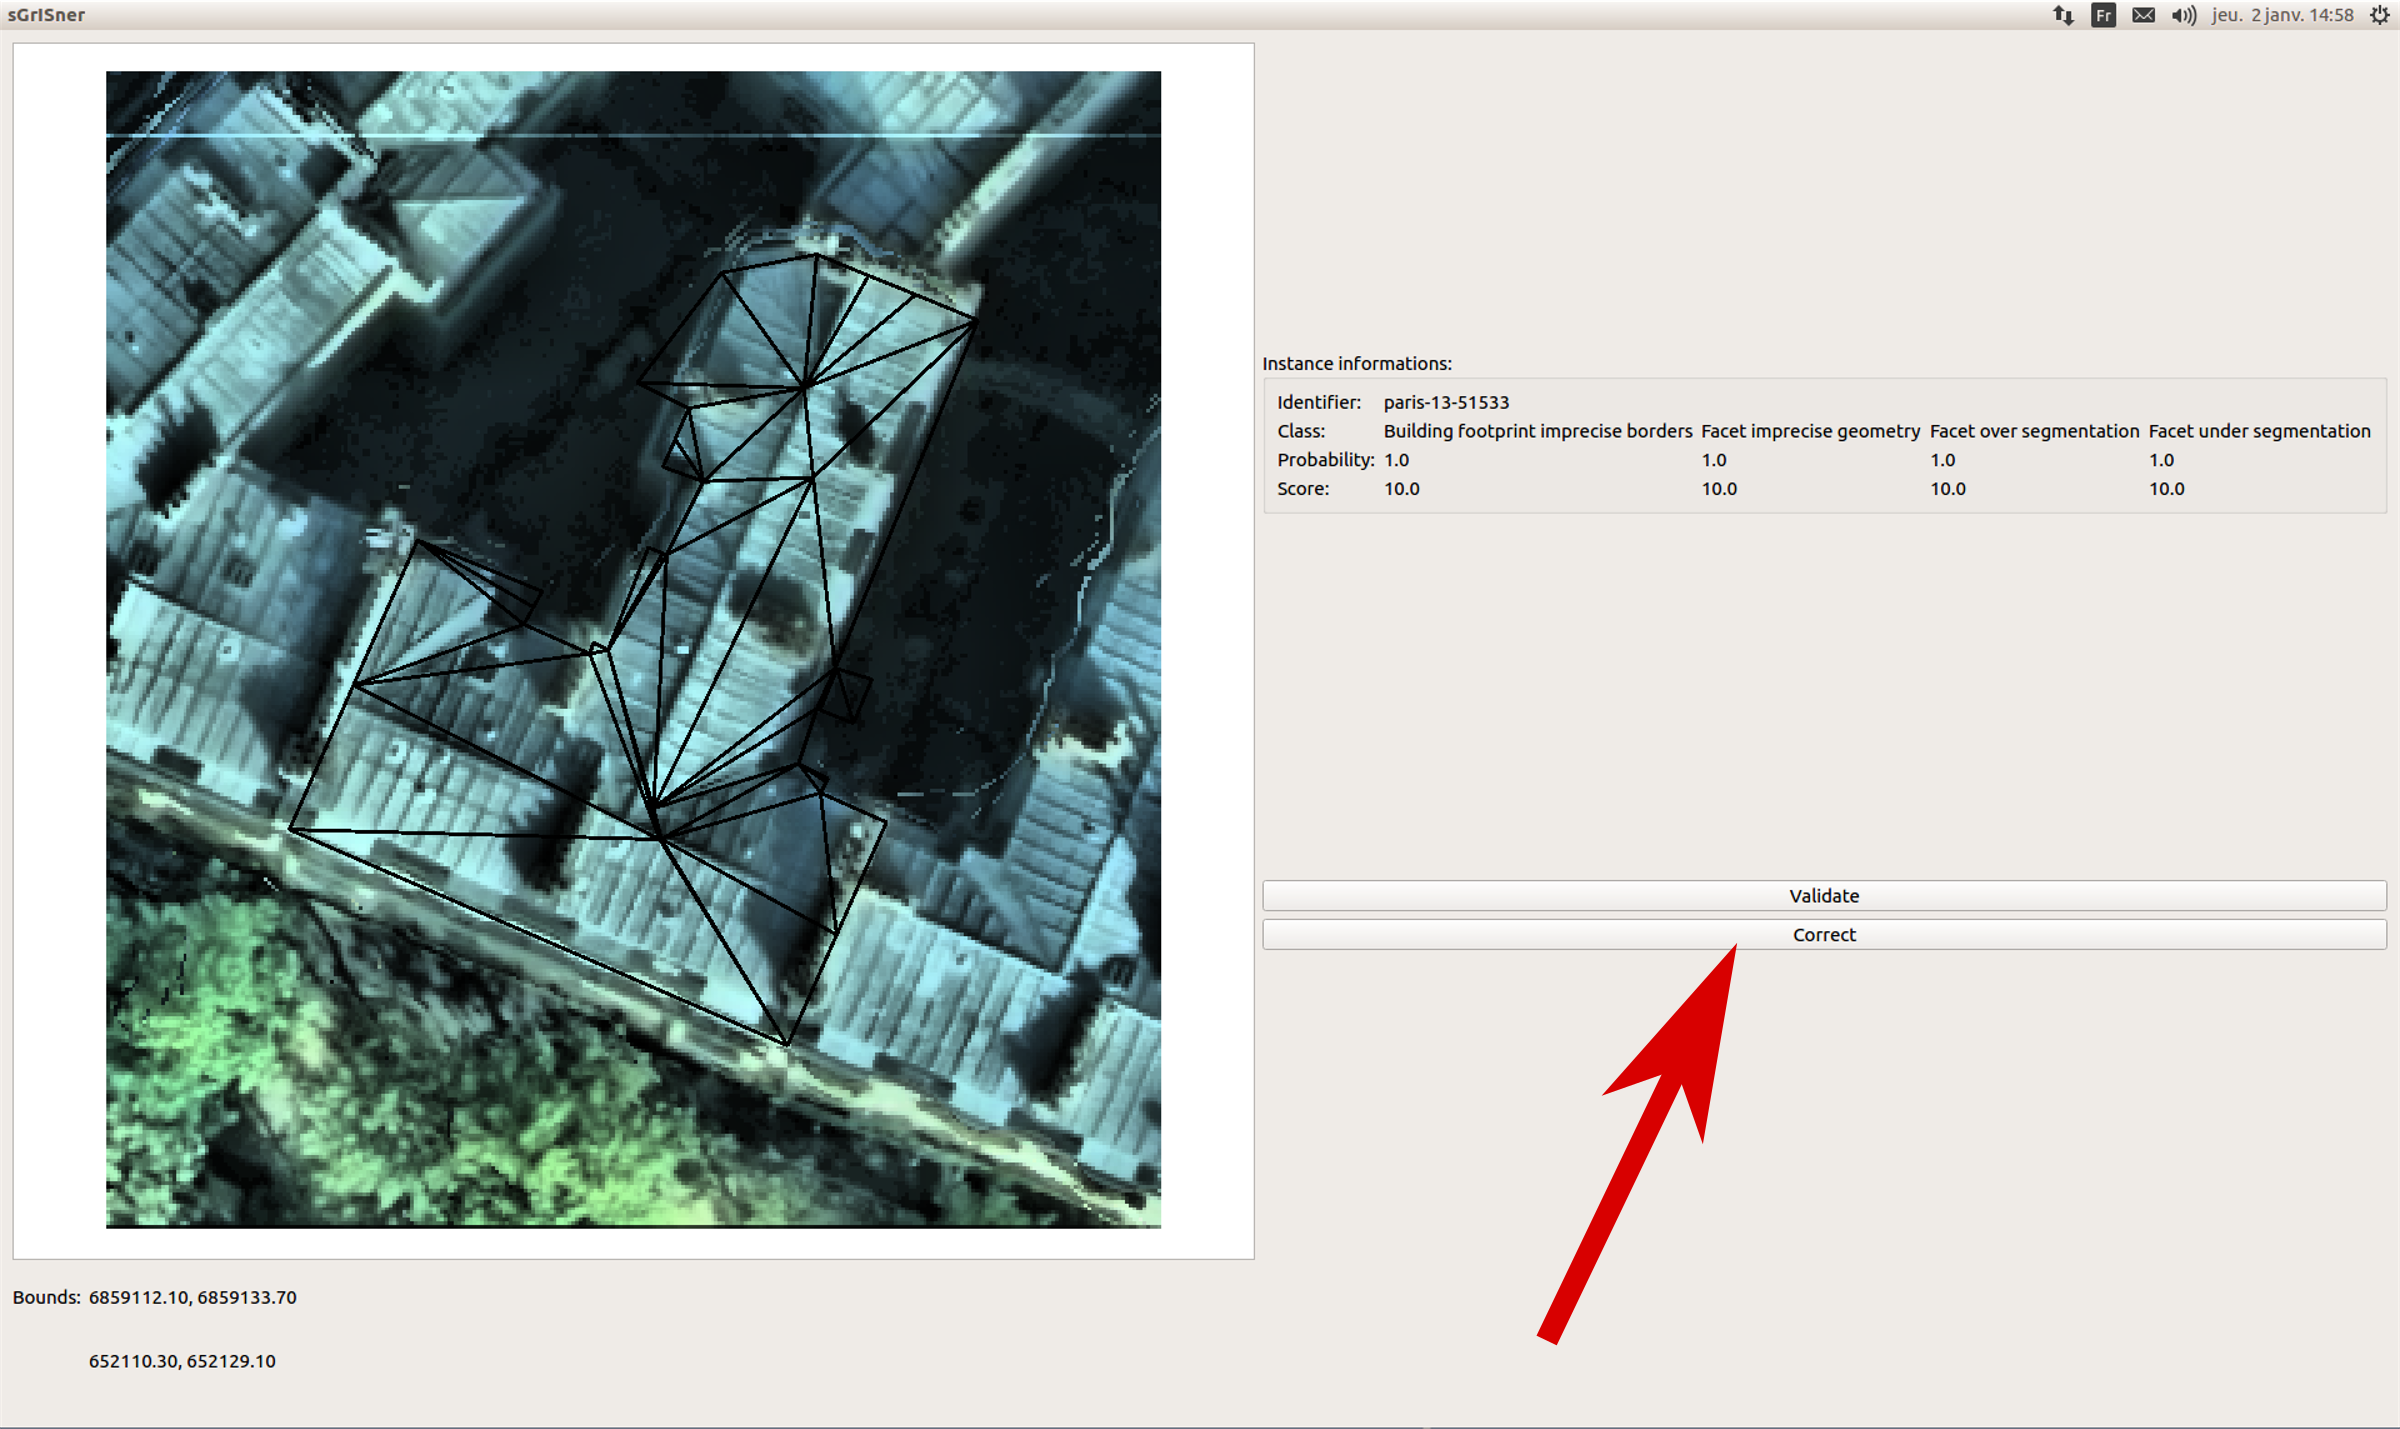
\includegraphics[width=\textwidth]{images/annotations/correction}
                    }{
                        \caption{
                            \label{subfig::correction}
                            The model is nadir projected and superposed to the orthoimage.
                            The operator either validates the error list or ammends it (red arrow).
                        }
                    }
                \end{subfloatrow}
                \vskip1em
                \begin{subfloatrow}
                    \centering
                    \ffigbox[\textwidth]{
                        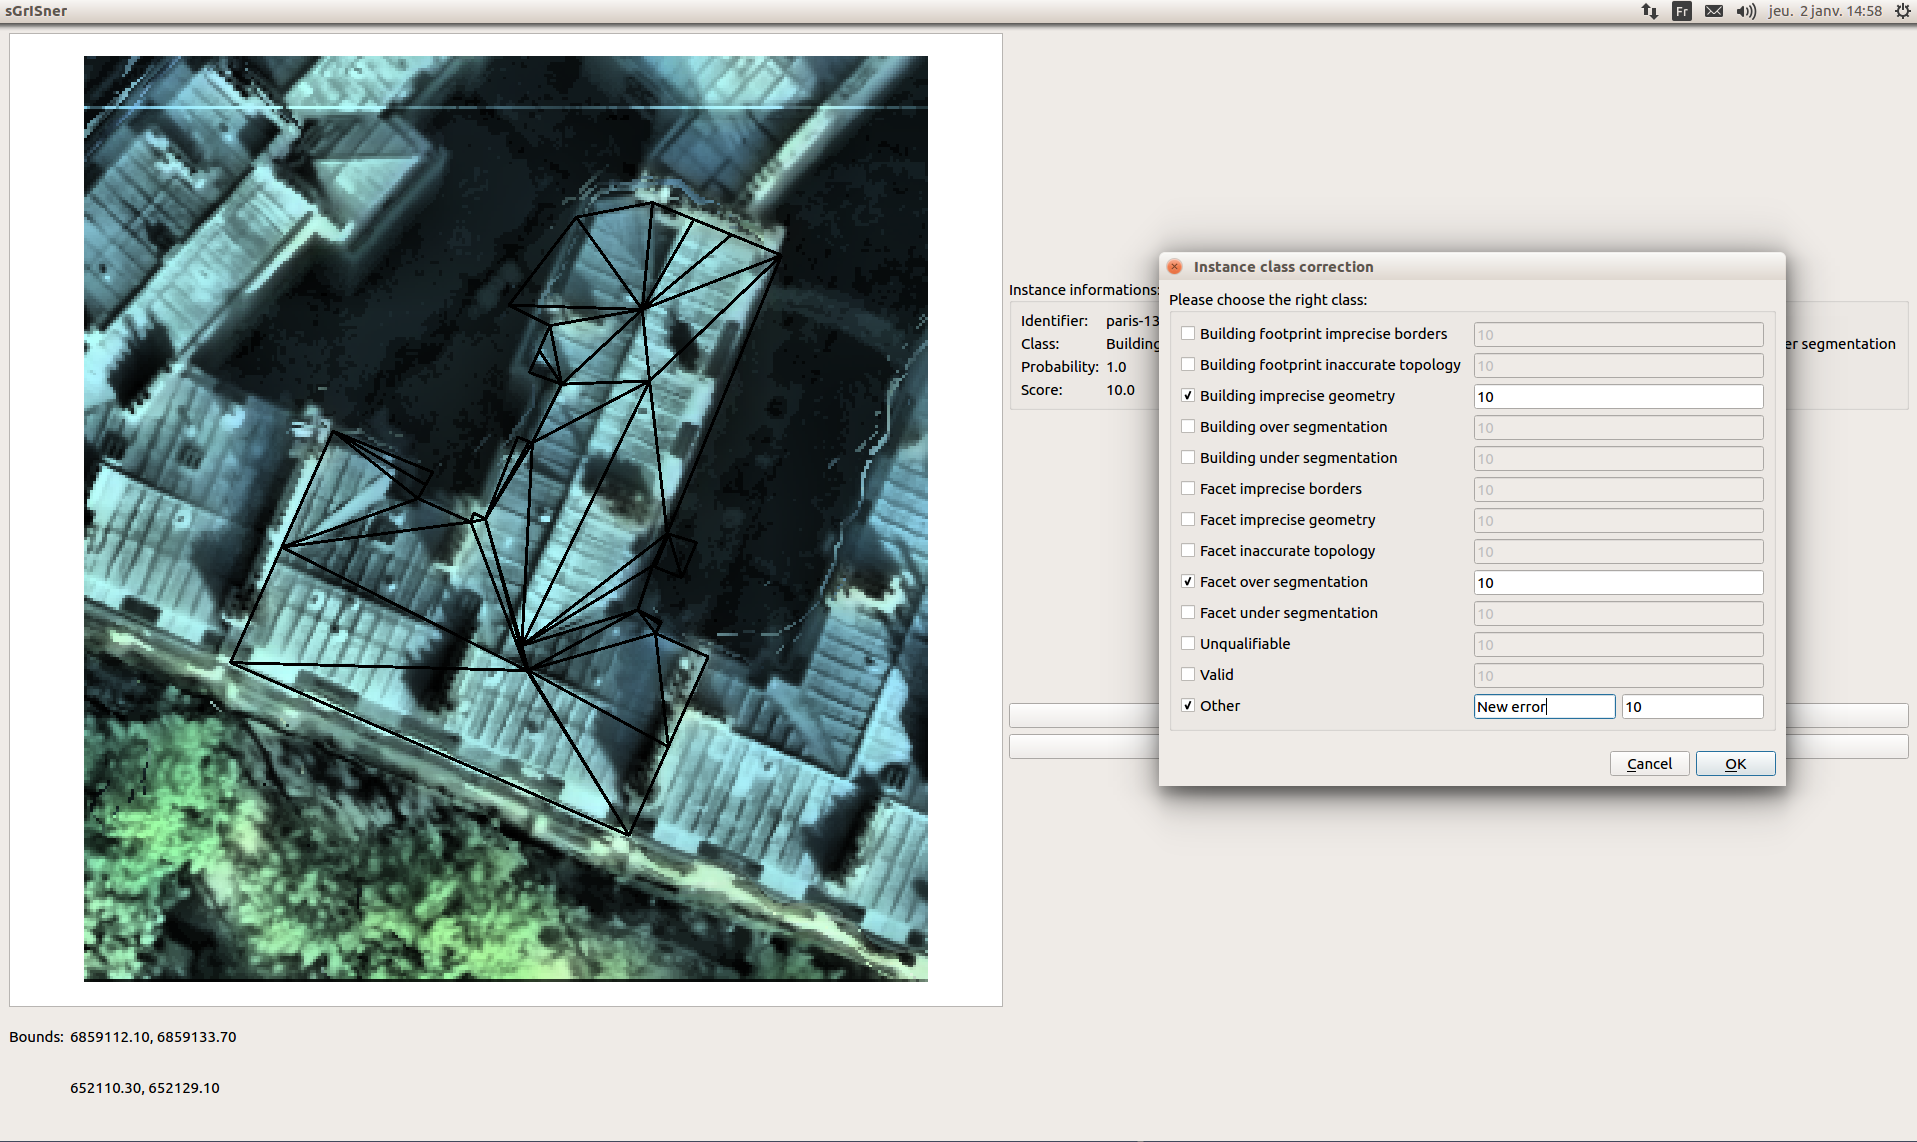
\includegraphics[width=\textwidth]{images/annotations/annotation}
                    }{
                        \caption{
                            \label{subfig::annotation}
                            The operator can ammend the error list from an established taxonomy or add a new error label if need be.
                            They can also assign confidence scores to each label.
                        }
                    }
                \end{subfloatrow}
            }{
                \caption{
                    \label{fig::annotation_tool}
                    Screenshots from the used annotation tool.
                }
            }
        \end{figure}

        Based on this annotation step modeling errors statistics were computed and compiled.
        These are depicted in Figure~\ref{fig::error_statistics}.\\

        \begin{figure}[htb]
            \centering
            \ffigbox[\textwidth]{
                \begin{subfloatrow}[2]
                    \centering
                    \ffigbox[.5\textwidth]{
                        \includestandalone[mode=buildnew, height=7.5cm]{figures/datasets/families_stats}
                    }{
                        \caption{
                            \label{subfig::family_errors}
                            Occurence statistics for error families and the \texttt{Unqualified} class computed for each area.
                        }
                    }
                    \ffigbox[.5\textwidth]{
                        \includestandalone[mode=buildnew, height=7.5cm]{figures/datasets/lod1_stats}
                    }{
                        \caption{
                            \label{subfig::lod1_errors}
                            Occurence statistics for \texttt{Building errors} depending on the area of  the scalability of the proposed approach under different scenarii..
                        }
                    }
                \end{subfloatrow}
                \vskip1em
                \begin{subfloatrow}
                    \centering
                    \ffigbox[\textwidth]{
                        \includestandalone[mode=buildnew, width=.7\textwidth]{figures/datasets/lod2_stats}
                    }{
                        \caption{
                            \label{subfig::lod2_errors}
                            Occurence statistics for \texttt{Facet errors} depending on the area of interest.
                        }
                    }
                \end{subfloatrow}
            }{
                \caption[
                    Detailed error statistics depending on the urban scenes.
                ]{
                    \label{fig::error_statistics}
                    Detailed error statistics depending on the urban scenes.
                    The height of bars indicates the frequency of each errors while the number of occurences is displayed above the bars.
                }
            }
        \end{figure}
        
        These statistics are first analysed depending on the family errors at the \texttt{finesse} = 2 level (cf. Figure~\ref{subfig::family_errors}).
        Due to the fact that geometrically inconsistent \gls{acr::3d} models were filtered out in a preprocessing (nadir projection) step, \texttt{Unqualifiable} buildings represent a small fraction of the dataset (less than \SI{7.5}{\percent}).
        Actually, the latter corresponds to the, partially or completly, occluded buildings that could not be qualified.
        Moreover, only a small fraction of buildings are \texttt{Valid}:
        57 (\SI{2.84}{\percent}) in \textbf{Elancourt}, 55 (\SI{7.35}{\percent}) for \textbf{Nantes} and 21 (\SI{4.39}{\percent}) in \textbf{Paris-13}.
        Most buildings are affected by the \texttt{Building Errors} family (over \SI{58.16}{\percent}) and the \texttt{Facet Errors} one (over \SI{75.94}{\percent}).\\

        At the \textbf{\gls{acr::efin}} level 3, two axes of analysis are possible.
        First, we group errors that are very frequent in the dataset.
        Over-segmentation errors (\texttt{FOS} and \texttt{BOS}), in both error families, are well represented ranging from \SIrange{38.9}{66.8}{\percent}.
        The same is true for \texttt{FIG} with a frequency from \SIrange{59.8}{80}{\percent}.
        \texttt{FIT}, on the other hand, are very rare in all the areas with ratios a little less than \SI{1.5}{\percent}.
        The rest have a presence ratio within the percentage interval of [10, 30].
        The errors that are rare are understandably going to have a negative impact on the learning process.\\
        
        Secondly, we can compare error frequency discrepancies depending on the studied scene.
        \textbf{Elancourt} is different compared to the relatively close sets \textbf{Nantes} and \textbf{Paris-13}, with regards to \texttt{BOS}, \texttt{BUS} and \texttt{BIT}.
        In fact, the last two areas are more densely urbanized than the first one exhibitting the same properties at \gls{acr::lod}-0.
        \texttt{BIB}, on the other hand, are equally distributed over the different datasets as this error type depends mostly on the input sensor data resolution independently of building types.\\
        At the facet level, \texttt{FIT} is also equally occuring across all the scenes different from the rest of \texttt{Facet errors}.
        In fact, \texttt{FOS} occurence ratio is related to the size of facets in urban scenes.
        Actually, the less complex roof structures are, the more big are facets and the more chance they have to be over segmented.
        Indeed, \textbf{Elancourt}, \textbf{Nantes} and \textbf{Paris-13} scenes are ordered in an ascending manner of their roof structure complexity.
        Conversely, in line with the previous analysis, \texttt{FUS} are less present in \textbf{Elancourt} than in \textbf{Nantes} which, in turn, contains less of the same error than \textbf{Paris-13}.
        \texttt{FIB} is distributed in the same manner as \texttt{FUS}.
        This is mainly due to the fact that the more a roof structure is complex the more precision errors are possible.
        \texttt{FIG} does not keep the same dynamic as its frequency keeps stable from \textbf{Elancourt} and \textbf{Nantes} but jumps considerably in \textbf{Paris-13}.
        This may be explained by the fact that the gap in \texttt{FUS} error ratios between \textbf{Paris-13} and \textbf{Nantes} is more important than that of \texttt{FOS} errors, contrarily to the same gaps for the same errors between \textbf{Nantes} and \textbf{Elancourt} which compensate each other.

\section{Baseline feature analysis}
    \label{sec::experiments::baseline_feature_analysis}
    In the previous sections, we have shown how our dataset of building models was assembled and how the urban scene composition influences modeling error statistics.
    We also specified in detail how each block of the pipeline was set up.
    At this stage, our aim is to prove the feasablity of the approach proposed in Chapter~\ref{chap::learned_evaluation}.
    As a consequence, for now, we limit ourselves to using the baseline features.\\

    First, in Section~\ref{subsec::experiments::baseline_feature_analysis::rmse}, the \gls{acr::rmse} is proven to be inadequate for detecting errors in our taxonomy.
    Secondly, prediction results from all possible configurations of baseline features are compared in Section~\ref{subsec::experiments::baseline_feature_analysis::vanilla}.
    Third and last, Section~\ref{subsec::experiments::baseline_feature_analysis::feature_importance} concludes the analysis by studying the feature importance, for all training zones.

    \subsection{\texorpdfstring{\acrlong*{acr::rmse}}{RMSE} predictive capacity}
        \label{subsec::experiments::baseline_feature_analysis::rmse}
        The \acrfull{acr::rmse} is the standard measure in most of \gls{acr::3d} modeling methods.
        As a consequence, we use it herein as a reference that our baseline is to be compared to.
        We train the classifier on Elancourt with the one dimensional feature vector containing the \gls{acr::rmse}.
        This scene was sufficient enough for our analysis.
        Mean test results are shown in Table~\ref{tab::rmse_results}.\\

        \begin{table}[htb]
            \footnotesize
            \begin{tabular}{c c c c c c c c c c}
                \toprule
                & \texttt{BOS} & \texttt{BUS} & \texttt{BIB} & \texttt{BIT} & \texttt{FOS} & \texttt{FUS} & \texttt{FIB} & \texttt{FIT} & \texttt{FIG} \\
                \midrule
                \(\bm{Rec}\) & 99.55 & 0.21 & 0 & 0 & 98.68 & 0.63 & 0 & 0 & 98.15 \\
                \midrule
                \(\bm{Prec}\) & 68.78 & 33.33 & --- & 0 & 66.60 & 0.25 & --- & 0 & 61.15 \\
                \midrule
                \(\bm{F_{score}}\) & 81.35 & 0.42 & 0 & 0 & 79.52 & 1.24 & 0 & 0 & 75.36 \\
                \midrule
                \(\bm{Acc}\) & 68.46 & 75.65 & 89.57 & 94.66 & 66.36 & 83.62 & 88.24 & 98.36 & 60.86 \\
                \bottomrule
            \end{tabular}
            \caption[
                \textbf{\gls{acr::efin}} 3 error prediction results using the \gls{acr::rmse} on \textbf{Elancourt}.
            ]{
                \label{tab::rmse_results}
                \textbf{\gls{acr::efin}} 3 error prediction results using the \gls{acr::rmse} on \textbf{Elancourt}.
                \(\bm{Acc}\) expresses the overall accuracy ratio.
            }
        \end{table}

        We can distinguish two groups of errors: 
        \begin{itemize}[label=\(\blacktriangleright\)]
            \item \texttt{BOS}, \texttt{FOS} and \texttt{FIG}: these have a high recall and a low precision and overall accuracy;
            \item \texttt{BUS}, \texttt{BIB}, \texttt{BIT}, \texttt{FUS}, \texttt{FIB} and \texttt{FIT}: these have low recall and precision ratios.
        \end{itemize}
        The first (\textit{resp.} second) group coincides exactly with errors that affect more (\textit{resp.} less) than half of the buildings.
        For this kind of errors, the classifier assigns to almost all samples the positive class.
        In fact, we end up with a high ratio of false positives (false alarms) and hence a high recall ratio that is coupled with a weak precision and overall accuracy.
        Exactly the inverse happens with the rest of the errors as we obtain a high percentage of false negative.
        We can safely conclude that the \gls{acr::rmse} is not able to detect errors defined in our taxonomy.

    \subsection{Vanilla experiments}
        \label{subsec::experiments::baseline_feature_analysis::vanilla}
        We tested the different feature configurations, at \textbf{\gls{acr::efin}} level 3 and in all urban zones\footnote{We train and test on different folds of the same scene.}.
        Mean precision and recall test results are reported in Table~\ref{tab::ablation_f3}.

        \begin{table}[htb]
            \footnotesize
            \begin{center}
                \begin{tabular}{| c | c c | c c | c c | c c |}
                    \hline
                    \multicolumn{9}{|c|}{\textbf{Elancourt}}\\
                    \hline
                    &\multicolumn{2}{c|}{\textbf{Geom.}} & \multicolumn{2}{c|}{\textbf{Geom. \(\oplus\) Hei.}} & \multicolumn{2}{c|}{\textbf{Geom. \(\oplus\) Im.}} & \multicolumn{2}{x{2.4cm}|}{\textbf{All}}\\
                    \cline{2-9}
                    & \(\bm{Rec}\) & \(\bm{Prec}\) &  \(\bm{Rec}\) & \(\bm{Prec}\) &  \(\bm{Rec}\) & \(\bm{Prec}\) &  \(\bm{Rec}\) & \(\bm{Prec}\) \\
                    \hline
                    \texttt{BOS} & \textbf{93.96} & \textbf{76.15} & 91.43 & 77.76 & 91.51 & 76.08 & 90.83 & 76.14 \\
                    \hline
                    \texttt{BUS} & 32.98 & 76.47 & \textbf{41.86} & \textbf{75.57} & 40.38 & 71.00 & 39.32 & 71.81 \\
                    \hline
                    \texttt{BIB} & 12.32 & 67.57 & 12.81 & 68.42 & \textbf{16.26} & \textbf{67.35} & 16.75 & 68.0 \\
                    \hline
                    \texttt{BIT} & \textbf{25.25} & \textbf{92.59} & 20.20 & 90.91 & 20.20 & 95.24 & 11.11 & 91.67 \\
                    \specialrule{.2em}{.1em}{.1em}
                    \texttt{FOS} & 98.91 & 99.07 & \textbf{98.91} & \textbf{99.30} & 98.99 & 98.84 & 98.91 & 98.84 \\
                    \hline
                    \texttt{FUS} & \textbf{1.90} & \textbf{54.55} & 0.63 & 66.67 & 1.61 & 50 & 1.27 & 66.67 \\
                    \hline
                    \texttt{FIB} & \textbf{9.17} & \textbf{87.5} & 0 & --- & 8.30 & 82.61 & 7.42 & 100 \\
                    \hline
                    \texttt{FIT} & 6.67 & 100 & \textbf{8.73} & \textbf{95.24} & 3.33 & 100 & 3.33 & 100 \\
                    \hline
                    \texttt{FIG} & \textbf{80.54} & \textbf{73.14} & 80.45 & 72.62 & 78.69 & 72.12 & 79.02 & 71.82 \\
                    \hline
                    \hline
                    \multicolumn{9}{|c|}{\textbf{Nantes}}\\
                    \hline
                    &\multicolumn{2}{c|}{\textbf{Geom.}} & \multicolumn{2}{c|}{\textbf{Geom. \(\oplus\) Hei.}} & \multicolumn{2}{c|}{\textbf{Geom. \(\oplus\) Im.}} & \multicolumn{2}{x{2.4cm}|}{\textbf{All}}\\
                    \cline{2-9}
                    & \(\bm{Rec}\) & \(\bm{Prec}\) &  \(\bm{Rec}\) & \(\bm{Prec}\) &  \(\bm{Rec}\) & \(\bm{Prec}\) &  \(\bm{Rec}\) & \(\bm{Prec}\) \\
                    \hline
                    \texttt{BOS} & \textbf{38.14} & \textbf{61.67} & 36.43 & 60.23 & 36.77 & 62.21 & 34.71 & 60.48 \\
                    \hline
                    \texttt{BUS} & 7.35 & 62.5 & 7.35 & 55.56 & \textbf{29.41} & \textbf{66.67} & 26.47 & 64.29 \\
                    \hline
                    \texttt{BIB} & 0 & --- & 0 & --- & \textbf{1.01} & \textbf{50.0} & \textbf{1.01} & \textbf{50.0} \\
                    \hline
                    \texttt{BIT} & 1.77 & 22.22 & \textbf{3.54} & \textbf{44.44} & 0 & 0 & 2.65 & 50.0 \\
                    \specialrule{.2em}{.1em}{.1em}
                    \texttt{FOS} & \textbf{98.54} & \textbf{98.13} & \textbf{98.54} & \textbf{98.13} & 98.33 & 97.92 & 98.12 & 97.91 \\
                    \hline
                    \texttt{FUS} & 27.62 & 55.24 & \textbf{27.62} & \textbf{59.18} & 24.76 & 54.74 & 23.33 & 53.85 \\
                    \hline
                    \texttt{FIB} & 37.80 & 62.0 & 36.59 & 63.16 & \textbf{49.39} & \textbf{60.90} & 46.39 & 60.90 \\
                    \hline
                    \texttt{FIT} & 0 & --- & 0 & --- & 0 & --- & 0 & --- \\
                    \hline
                    \texttt{FIG} & 86.32 & 78.09 & \textbf{86.77} & \textbf{78.02} & 84.53 & 78.71 & 83.86 & 78.08 \\
                    \hline
                    \hline
                    \multicolumn{9}{|c|}{\textbf{Paris-13}}\\
                    \hline
                    &\multicolumn{2}{c|}{\textbf{Geom.}} & \multicolumn{2}{c|}{\textbf{Geom. \(\oplus\) Hei.}} & \multicolumn{2}{c|}{\textbf{Geom. \(\oplus\) Im.}} & \multicolumn{2}{x{2.4cm}|}{\textbf{All}}\\
                    \cline{2-9}
                    & \(\bm{Rec}\) & \(\bm{Prec}\) &  \(\bm{Rec}\) & \(\bm{Prec}\) &  \(\bm{Rec}\) & \(\bm{Prec}\) &  \(\bm{Rec}\) & \(\bm{Prec}\) \\
                    \hline
                    \texttt{BOS} & 45.54 & 65.25 & 46.53 & 68.61 & \textbf{50.0} & \textbf{68.24} & 46.53 & 70.15 \\
                    \hline
                    \texttt{BUS} & 6.35 & 66.67 & 7.94 & 71.43 & \textbf{22.22} & \textbf{77.78} & 7.94 & 62.5 \\
                    \hline
                    \texttt{BIB} & 0 & --- & 0 & --- & 0 & 0 & 0 & --- \\
                    \hline
                    \texttt{BIT} & \textbf{2.63} & \textbf{50.0} & 0 & --- & 1.32 & 50.0 & 0 & 0 \\
                    \specialrule{.2em}{.1em}{.1em}
                    \texttt{FOS} & 97.19 & 97.19 & 97.19 & 97.19 & \textbf{97.59} & \textbf{98.38} & 97.19 & 97.19 \\
                    \hline
                    \texttt{FUS} & \textbf{85.09} & \textbf{75.0} & 84.36 & 74.12 & 85.09 & 74.52 & 84.36 & 74.12 \\
                    \hline
                    \texttt{FIB} & 53.47 & 62.10 & 51.39 & 61.67 & \textbf{53.47} & \textbf{63.11} & 52.78 & 61.79 \\
                    \hline
                    \texttt{FIT} & 0 & --- & 0 & --- & 0 & --- & 0 & --- \\
                    \hline
                    \texttt{FIG} & 97.65 & 84.62 & \textbf{98.96} & \textbf{84.79} & 97.65 & 84.62 & \textbf{98.96} & \textbf{84.79} \\
                    \hline
                \end{tabular}
            \end{center}
            \caption[
                Baseline feature ablation study results preformed on the three areas at \textbf{\gls{acr::efin}} level 3.
            ]{
                \label{tab::ablation_f3}
                Baseline feature ablation study results preformed on the three areas at \textbf{\gls{acr::efin}} level 3.
                Test results are expressed in percentage.
                All \texttt{atomic} errors are considered over all possible configurations.
                Results in bold indicate the feature configuration with the highest F-score.
            }
        \end{table}

        In Table~\ref{tab::all_f-scores_ablation_f3_viz}, results are classified depending on the F-score using a color scheme.
        We can see how \texttt{FOS} and \texttt{FIG} are always well detected.
        This is mainly due to the fact that they are very frequent in all datasets (cf. Figure~\ref{fig::error_statistics}).
        The same reason explains why \texttt{BOS} is well detected in \textbf{Elancourt}, as well as \texttt{FUS} and \texttt{FIB} are in \textbf{Paris-13}.
        Understandably, rare errors are difficult to detect as shown by \texttt{FIT} on the three zones for instance.

        \begin{table}[htb]
            \footnotesize
            \centering
            \renewcommand{\arraystretch}{1.5}
            \begin{center}
                \begin{tabular}{| c | x{1.5cm} x{1.5cm} x{1.5cm} x{1.5cm} |}
                    \hline
                    & \multicolumn{4}{c|}{\textbf{Elancourt}}\\
                    \hline
                    &\textbf{Geom.} & \textbf{Geom. \(\oplus\) Hei.} & \textbf{Geom. \(\oplus\) Im.} & \textbf{All}\\
                    \hline
                    \texttt{BOS} & \cellcolor{GAIN2535} & \cellcolor{GAIN2535} & \cellcolor{GAIN2535} & \cellcolor{GAIN2535} \\
                    \hline
                    \texttt{BUS} & \cellcolor{LOSS0515} & \cellcolor{LOSS0515} & \cellcolor{LOSS0515} & \cellcolor{LOSS0515} \\
                    \hline
                    \texttt{BIB} & \cellcolor{LOSS2535} & \cellcolor{LOSS2535} & \cellcolor{LOSS2535} & \cellcolor{LOSS2535} \\
                    \hline
                    \texttt{BIT} & \cellcolor{LOSS2535} & \cellcolor{LOSS2535} & \cellcolor{LOSS2535} & \cellcolor{LOSS2535} \\
                    \specialrule{.2em}{.1em}{.1em}
                    \texttt{FOS} & \cellcolor{GAIN45} & \cellcolor{GAIN45} & \cellcolor{GAIN45} & \cellcolor{GAIN45} \\
                    \hline
                    \texttt{FUS} & \cellcolor{LOSS3545} & \cellcolor{LOSS3545} & \cellcolor{LOSS3545} & \cellcolor{LOSS3545} \\
                    \hline
                    \texttt{FIB} & \cellcolor{LOSS2535} & \cellcolor{LOSS3545} & \cellcolor{LOSS2535} & \cellcolor{LOSS3545} \\
                    \hline
                    \texttt{FIT} & \cellcolor{LOSS3545} & \cellcolor{LOSS2535} & \cellcolor{LOSS3545} & \cellcolor{LOSS3545} \\
                    \hline
                    \texttt{FIG} & \cellcolor{GAIN2535} & \cellcolor{GAIN2535} & \cellcolor{GAIN2535} & \cellcolor{GAIN2535} \\
                    \hline
                    \hline
                    & \multicolumn{4}{c|}{\textbf{Nantes}}\\
                    \hline
                    &\textbf{Geom.} & \textbf{Geom. \(\oplus\) Hei.} & \textbf{Geom. \(\oplus\) Im.} & \textbf{All}\\
                    \hline
                    \texttt{BOS} & \cellcolor{LOSS0515} & \cellcolor{LOSS0515} & \cellcolor{LOSS0515} & \cellcolor{LOSS2535} \\
                    \hline
                    \texttt{BUS} & \cellcolor{LOSS3545} & \cellcolor{LOSS3545} & \cellcolor{LOSS2535} & \cellcolor{LOSS2535} \\
                    \hline
                    \texttt{BIB} & \cellcolor{LOSS3545} & \cellcolor{LOSS3545} & \cellcolor{LOSS3545} & \cellcolor{LOSS3545} \\
                    \hline
                    \texttt{BIT} & \cellcolor{LOSS3545} & \cellcolor{LOSS3545} & \cellcolor{LOSS3545} & \cellcolor{LOSS3545} \\
                    \specialrule{.2em}{.1em}{.1em}
                    \texttt{FOS} & \cellcolor{GAIN45} & \cellcolor{GAIN45} & \cellcolor{GAIN45} & \cellcolor{GAIN45} \\
                    \hline
                    \texttt{FUS} & \cellcolor{LOSS2535} & \cellcolor{LOSS2535} & \cellcolor{LOSS2535} & \cellcolor{LOSS2535} \\
                    \hline
                    \texttt{FIB} & \cellcolor{LOSS0515} & \cellcolor{LOSS0515} & \cellcolor{LOSS0515} & \cellcolor{LOSS0515} \\
                    \hline
                    \texttt{FIT} & \cellcolor{LOSS3545} & \cellcolor{LOSS3545} & \cellcolor{LOSS3545} & \cellcolor{LOSS3545} \\
                    \hline
                    \texttt{FIG} & \cellcolor{GAIN2535} & \cellcolor{GAIN2535} & \cellcolor{GAIN2535} & \cellcolor{GAIN2535} \\
                    \hline
                    \hline
                    & \multicolumn{4}{c|}{\textbf{Paris-13}}\\
                    \hline
                    &\textbf{Geom.} & \textbf{Geom. \(\oplus\) Hei.} & \textbf{Geom. \(\oplus\) Im.} & \textbf{All}\\
                    \hline
                    \texttt{BOS} & \cellcolor{LOSS0515} & \cellcolor{GAIN1525} & \cellcolor{GAIN1525} & \cellcolor{GAIN1525} \\
                    \hline
                    \texttt{BUS} & \cellcolor{LOSS3545} & \cellcolor{LOSS3545} & \cellcolor{LOSS2535} & \cellcolor{LOSS3545} \\
                    \hline
                    \texttt{BIB} & \cellcolor{LOSS3545} & \cellcolor{LOSS3545} & \cellcolor{LOSS3545} & \cellcolor{LOSS3545} \\
                    \hline
                    \texttt{BIT} & \cellcolor{LOSS3545} & \cellcolor{LOSS3545} & \cellcolor{LOSS3545} & \cellcolor{LOSS3545} \\
                    \specialrule{.2em}{.1em}{.1em}
                    \texttt{FOS} & \cellcolor{GAIN45} & \cellcolor{GAIN45} & \cellcolor{GAIN45} & \cellcolor{GAIN45} \\
                    \hline
                    \texttt{FUS} & \cellcolor{GAIN2535} & \cellcolor{GAIN2535} & \cellcolor{GAIN2535} & \cellcolor{GAIN2535} \\
                    \hline
                    \texttt{FIB} & \cellcolor{GAIN1525} & \cellcolor{GAIN1525} & \cellcolor{GAIN1525} & \cellcolor{GAIN1525} \\
                    \hline
                    \texttt{FIT} & \cellcolor{LOSS3545} & \cellcolor{LOSS3545} & \cellcolor{LOSS3545} & \cellcolor{LOSS3545} \\
                    \hline
                    \texttt{FIG} & \cellcolor{GAIN45} & \cellcolor{GAIN45} & \cellcolor{GAIN45} & \cellcolor{GAIN45} \\
                    \hline
                \end{tabular}
            \end{center}
            \renewcommand{\arraystretch}{1}
            \caption[
                F-scores vizualization for ablation results at \textbf{\gls{acr::efin}} level 3 with baseline features.
            ]{
                \label{tab::all_f-scores_ablation_f3_viz}
                F-scores vizualization for ablation results at \textbf{\gls{acr::efin}} level 3 with baseline features.
                These are deduced from Table~\ref{tab::all_f-scores_ablation_f3}.
                The color indicates the how well detected a label is: 
                \textcolor{LOSS3545}{\(\blacksquare\)}: [\SIrange[range-phrase={, }]{0}{15}{\percent})--
                \textcolor{LOSS2535}{\(\blacksquare\)}: [\SIrange[range-phrase={, }]{15}{45}{\percent}) --
                \textcolor{LOSS0515}{\(\blacksquare\)}: [\SIrange[range-phrase={, }]{45}{55}{\percent}) --
                \textcolor{GAIN1525}{\(\blacksquare\)}: [\SIrange[range-phrase={, }]{55}{70}{\percent})--
                \textcolor{GAIN2535}{\(\blacksquare\)}: [\SIrange[range-phrase={, }]{70}{85}{\percent})--
                \textcolor{GAIN45}{\(\blacksquare\)}: [\SIrange[range-phrase={, }]{85}{100}{\percent}].
            }
        \end{table}

        \begin{figure}[htb]
            \centering
            \ffigbox[\FBwidth]{
                \begin{subfloatrow}[2]
                    \ffigbox[\FBwidth]{
                        \includestandalone[mode=buildnew, height=7.5cm]{figures/results/ablation/building}
                    }{
                        \caption{
                            \label{subfig::f_score_ablation_f3_building}
                            \texttt{Building errors.}
                        }
                    }
                    \ffigbox[\FBwidth]{
                        \includestandalone[mode=buildnew, height=7.5cm]{figures/results/ablation/facet}
                    }{
                        \caption{
                            \label{subfig::f_score_ablation_f3_facet}
                            \texttt{Facet errors.}
                        }
                    }
                \end{subfloatrow}
            }{
                \caption[
                    Visualizing mean F-score and standard deviation for the feature ablation study.
                ]{
                    \label{fig::f_score_ablation_f3}
                    Visualizing mean F-score and standard deviation for the feature ablation study.
                    Details are reported in Table~\ref{tab::f_score_ablation_f3}.
                }
            }
        \end{figure}

        F-scores are averaged across all feature configurations and represented in Figure~\ref{fig::f_score_ablation_f3}.
        The first thing we can observe is the fact that geometric features alone give comparable results to ones where extrinsic modalities are added.
        This was the case for most errors as confirmed by the low variance in F-score.
        However, in some exceptional cases, adding more modalities impacts greatly the results as shown in Table~\ref{tab::all_f-scores_ablation_f3}.
        The first case regards \texttt{BUS}.
        In fact, on \textbf{Elancourt}, height and image based features both contribute to an increase of around \SI{6}{\percent} in F-score.
        This can be explained by the fact that a lot of under-segmented building models have different heights which reflects easily on height based features.
        Similar behaviour occurs for \textbf{Nantes} and \textbf{Paris-13} with image based features driving at least a \SI{20}{\percent} jump in F-score.
        In fact, buildings could be identified by their roof texture or color, as depicted in Figure~\ref{subfig::bus_2d}.
        As a consequence, image based features are instrumental in detecting the discrepancy between two under-segmented buildings, especially in dense uniform settings.
        The second and less important example is \texttt{FIB} on \textbf{Nantes} where image based features adds around \SI{10}{\percent} in F-score as designed in Section~\ref{subsec::learned_evaluation::baseline::image}.
        Last comes the case of \texttt{BIT}, on \textbf{Elancourt}, which performs at least \SI{6}{\percent} worse when adding more modalities.

        This can be actually interpreted by the fact that geometric features, take into account intrinsic attributes of a building model.
        These features could, in turn, be intuitively related to the type of building they describe.
        Consequently, the big role that this kind of features plays in detecting errors implies that the existence of a defect is highly correlated to the type of model it affects.\\
        This is, in fact, expected for errors of topological nature as the geometric structure of the model is assessed.
        As an example, we can see how \texttt{BOS} is better detected on \textbf{Elancourt} and \textbf{Nantes} based on geometric features only.
        Extrinsic features, on the other hand, act more as clues in predicting these types of errors as discussed with \texttt{BUS} in the previous paragraph.\\

        Conversely, the image and height based features are expected to yield at least as good results as the intrinsic features alone for fidelity defects.
        In fact, in Table~\ref{tab::ablation_f3}, \texttt{BIB} as well as \texttt{FIB} and \texttt{FIG} are better detected, in terms of F-score, when adding height or image based modalities.
        The exception is \texttt{FIB} and \texttt{FIG} on \textbf{Elancourt} where only geometric features yielded better results.
        This may be explained by the fact that the baseline features are not rich enough and the shear number of training instances in \textbf{Elancourt} was sufficient to link building model types to the occurence of such errors.\\

        Figure~\ref{fig::f_score_ablation_f3} shows that all \texttt{Building errors} labels are better detected on \textbf{Elancourt}.
        Moreover, we can even establish that the more the urban scene is dense the more difficult \gls{acr::lod}-0 \(\cup\) \gls{acr::lod}-1 errors detection becomes.
        There is one exception where \texttt{BOS} existence is slightly better predicted on \textbf{Paris-13} than on \textbf{Nantes}.
        This may be attributed to the low number of training samples on both these zones, as they are not sufficiently representative of the actual scenes.
        On the other hand, \texttt{Facet errors} F-scores are proportional to the density of the studied urban scene, minding two exceptions.
        \texttt{FOS} and \texttt{FIT} F-scores are actually stable across the different urban areas suffering only from slight decreases that can be attributed to noise.
        This can be due to the fact that \texttt{FOS} is highly frequent in all urban scenes and so easily predictable that F-scores cannot get any better. 
        Conversely, \texttt{FIT} are so rare (cf. Figure~\ref{subfig::lod2_errors}) their existance is barely predictable.

    \subsection{Feature importance}
        \label{subsec::experiments::baseline_feature_analysis::feature_importance}
        \begin{figure}[htb]
            \centering
            \ffigbox[\FBwidth]{
                \begin{subfloatrow}
                    \ffigbox[\FBwidth]{
                        \includestandalone[mode=buildnew, height=.23\textheight]{figures/results/ablation/feature_importance/building}
                    }{
                        \caption{
                            \label{subfig::feature_importances_rf_bl_building}
                            \texttt{Building errors.}
                        }
                    }
                    \ffigbox[\FBwidth]{
                        \includestandalone[mode=buildnew, height=.23\textheight]{figures/results/ablation/feature_importance/facet}
                    }{
                        \caption{
                            \label{subfig::feature_importances_rf_bl_facet}
                            \texttt{Facet errors.}
                        }
                    }
                \end{subfloatrow}
            }{
                \caption[
                    Modality importance computed by stacking single feature importances retrieved from the \gls{acr::rf} classifier.
                ]{
                    \label{fig::feature_importances_rf_bl}
                    Modality importance computed by stacking single feature importances retrieved from the \gls{acr::rf} classifier.
                    The first (\textit{resp.} second and third) column represents \textbf{Elancourt} (\textit{resp.} \textbf{Nantes} and \textbf{Paris-13}).
                }
            }
        \end{figure}
        
        \gls{acr::rf} classifiers can easily infer feature importances at training time.
        These were here computed and aggregated by modality in all urban scenes (cf. Figure~\ref{fig::feature_importances_rf_bl}).\\

        At first, we observe how important individual attributes are before being gathered.
        For geometric features, all attributes are equally important.
        However, concerning image and height based features, only a few are relevant (i.e., they have a higher feature importance ratio).
        Indeed, these few attributes correspond to the highest and lowest values of the histograms.
        As described earlier, image and height features consist of a histogram of distances between the model and the real measured signals:
        vector cosine similarity, for the first, and the \(L_2\) norm for the last.
        It is clear that the presence of errors would result in saturating the high values in the histogram, while an absence of defects would imply a big number of low values.
        This is one intuitive explaination of this observed phenomenon.\\
        
        In a second time, we notice that no modality is more important than the others, contrarily to what was observed in Table~\ref{tab::ablation_f3}.
        In fact, as shown in Section~\ref{subsec::experiments::baseline_feature_analysis::vanilla}, for most \texttt{atomic} errors, test results using geometric features are comparable to those obtained with more modalities.
        However, during training, all modalities are relevant with importance ratios approximating \num[fraction-function = \sfrac]{1/3} as shown in Figure~\ref{fig::feature_importances_rf_bl}.
        As a consequence, for subsequent experimentations all configurations are taken into consideration.

    \subsection{Summary}
        \label{subsec::experiments::baseline_feature_analysis::summary}
        In this section, we have used the \gls{acr::rf} classifier on two types of features: a simple \gls{acr::rmse} and the custom build baseline features.
        From the experimental results, we have learned that:
        \begin{itemize}[label=\(\blacktriangleright\)]
            \item The \gls{acr::rmse} fails completly to predict errors defined in our taxonomy;
            \item \texttt{Building errors} are better detected on \textbf{Elancourt} than on the other scenes;
            \item \texttt{FOS} is very well detected with over \SI{95}{\percent} in F-score, over all areas of interest;
            \item Except \texttt{FOS}, the more the urban zone is dense the better \texttt{Facet erros} are detected;
            \item Rare errors such as \texttt{BIT} and \texttt{FIT} (on all urban areas) are poorly detected;
            \item Geometric features alone are, with a small margin, as good as the other extrinsic based configurations for error detection;
            \item Consequently, the building type is a good indicator for error detection in the same area;
            \item \texttt{BUS} is the only error that the other modalities are better at with a large gap;
            \item Although, in most cases, not improving error prediction, external data based modalities are as important as geometric features.
        \end{itemize}

\section{Scalability analysis}
    \label{sec::experiments::scalability}
    In the previous section, error detection was proven to depend on the scene composition.
    This fact motivates studying training the classifier and testing prediction on different scenes.
    The goal is to prove the resilience of error detection to unseen urban scenes.
    As the annotation process requires a lot of effort, this trait is crucial to guarantee the scalability of this method under the \textbf{large-scale} constraint.\\

    Different configurations are possible, as depicted in Figure~\ref{fig::scalability_study}.
    In the first type of experiments, we train on one urban scene and test on another one.
    The goal is to examine the \texttt{transferability} of the classifier model.
    Experimental results are reported and analyzed in Section~\ref{subsec::experiments::scalability::transferability}.
    In a second configuration, the classifier is trained on two scenes and tested on the last one: the objective is to investigate the classifier \texttt{generalization}.
    The results of such experiments are shown in Section~\ref{subsec::experiments::scalability::generalization}.
    The last experiment class, whose results are presented in Section~\ref{subsec::experiments::scalability::representativeness}, targets the \texttt{representativeness} of a single 3-area dataset by trying multiple train-test split sizes.\\

    \begin{figure}[htbp]
        \ffigbox[\FBwidth]{
            \includestandalone[mode=buildnew, width=.8\textwidth]{figures/scalabitity_graph}
        }
        {
            \caption[
                A graph representing possible experiments: arrow origins represent training scenes while test ones are depicted as targets.
            ]{
                \label{fig::scalability_study}
                A graph representing possible experiments: arrow origins represent training scenes while test ones are depicted as targets.
                \(Z_i, i=1,2,3\) represent the urban zones.
                All these nodes are assembled in one, meaning that all urban scenes were aggregated in on train/test node.
                The numbers indicate in which section each experiment is analyzed.
            }
        }
    \end{figure}

    \subsection{Transferability study}
        \label{subsec::experiments::scalability::transferability}
        In this configuration, we test how transferable the learned classifiers are from one urban scene to another.
        We train on a zone $Z_i$ and test on another one $Z_j$.
        We will denote each transferability experiment by the couple $(Z_i, Z_j)$ or by $Z_i \rightarrow Z_j$.
        Six transferability couples are possible and are tested with all possible feature configurations.
        Mean and standard deviation of F-scores are plotted, for each label and experiment, in Figure~\ref{fig::f_score_transferability_f3}.
        For more details, refer to Tables~\ref{tab::transferability_f3} and~\ref{tab::all_f-scores_transferability_f3}, which compiles all precision, recall and F-score test results.\\
        
        \thisfloatsetup{subfloatrowsep=none}
        \begin{figure}[htbp]
            \ffigbox[\textwidth]{
                \begin{subfloatrow}
                    \centering
                    \ffigbox[\textwidth]{
                        \includestandalone[mode=buildnew, width=\textwidth]{figures/results/transferability/building}
                    }{
                        \caption{
                            \label{subfig::f_score_transferability_f3_building}
                            \texttt{Building errors.}
                        }
                    }
                \end{subfloatrow}
                \vskip2em
                \begin{subfloatrow}
                    \ffigbox[\textwidth]{
                        \includestandalone[mode=buildnew, width=\textwidth]{figures/results/transferability/facet}
                    }{
                        \caption{
                            \label{subfig::f_score_transferability_f3_facet}
                            \texttt{Facet errors.}
                        }
                    }
                \end{subfloatrow}
            }{
                \caption[
                    Mean F-score and standard deviation for the transferability study.
                ]{
                    \label{fig::f_score_transferability_f3}
                    Mean F-score and standard deviation for the transferability study.
                    \textbf{El.} (\textit{resp.} \textbf{Na.} and \textbf{P13.}) stand for \textbf{Elancourt} (\textit{resp.} \textbf{Nantes} and \textbf{Paris-13}).
                    This is a vizualization of results reported in Table~\ref{tab::f_score_transferability_f3}.
                }
            }
        \end{figure}

        \subparagraph{\texttt{Coherence} study.}
            First, a \texttt{coherence} analysis is performed.
            We compare the results of the transferability experiments to the ablation results with the same training scene.
            This is achieved by looking, for a given area $Z_i$ in all couples $(Z_i, Z_j)_{\forall j \neq i}$, at the differences between Tables~\ref{tab::all_f-scores_transferability_f3} and~\ref{tab::all_f-scores_ablation_f3}.
            The goal is to see to which extent the test and training zone are similar.\\

            \begin{figure}[htb]
                \centering
                \includestandalone[mode=buildnew, width=.9\textwidth]{figures/results/comparison_bar}
                \caption[
                    Color scheme used for F-score comparisons in this study.
                ]{
                    \label{fig::comparison_bar}
                    Color scheme used for F-score comparisons in this study.
                    When two null F-scores are compared, the cell is colored in white.
                }
            \end{figure}

            All these comparisons are provided in Table~\ref{tab::transferability_comparison}.
            A color scheme was devised to encode the amplitude of change and is illustrated in Figure~\ref{fig::comparison_bar}.
            The resemblance between \textbf{Paris-13} and \textbf{Nantes} are striking.
            In fact, when training on one of the two zones and testing on \textbf{Elancourt}, out of the nine labels only two are different.
            \texttt{BUS} has a gain between \SIrange[range-phrase={ and }]{5}{15}{\percent} when trained on \textbf{Paris-13} while its F-score records a drop in the range \SIrange{-15}{-5}{\percent} if trained on \textbf{Nantes}.
            \texttt{FUS}, in contrast, looses between \SIrange[range-phrase={ and }]{-45}{-35}{\percent} when trained on \textbf{Paris-13} and \SIrange[range-phrase={ and }]{-35}{-25}{\percent} for \textbf{Nantes}.\\
            Conversely when training on \textbf{Elancourt} and testing on the other two areas, the comparisons are not as identical as before.
            However, from a general standpoint, we can see how the \texttt{building errors} are always affected by losses when testing on both \textbf{Paris-13} and \textbf{Nantes}.
            Except for \texttt{FIT}, the inverse situation is obseved for \texttt{Facet errors} where labels are either better detected or stable.

        \begin{table}[htbp]
            \footnotesize 
            \centering
            \renewcommand{\arraystretch}{2}
            \begin{tabular}{| c | c | c c c c |c c c c c|}
                \hline
                && \texttt{BOS} & \texttt{BUS} & \texttt{BIB} & \texttt{BIT} & \texttt{FOS} & \texttt{FUS} & \texttt{FIB} & \texttt{FIT} & \texttt{FIG}\\
                \hline
                \multirow{6}{*}{\rotatebox{90}{\texttt{Coherence}}} & \textbf{El.} \(\rightarrow\) \textbf{Na.} & \cellcolor{LOSS2535} & \cellcolor{LOSS1525} \textbf{All} & \cellcolor{LOSS2535} & \cellcolor{LOSS1525} \textbf{All} & \cellcolor{STBL} & \cellcolor{GAIN1525} \textbf{Im.} & \cellcolor{GAIN3545} \textbf{Im.} & \cellcolor{STBL} \textbf{Im.} & \cellcolor{GAIN0515} \\
                & \textbf{El.} \(\rightarrow\) \textbf{P13} & \cellcolor{LOSS1525} & \cellcolor{LOSS1525} \textbf{Im.} & \cellcolor{LOSS1525} & \cellcolor{LOSS2535} & \cellcolor{STBL} & \cellcolor{GAIN3545} \textbf{Im.} & \cellcolor{GAIN2535} \textbf{Im.} & \cellcolor{LOSS1525} & \cellcolor{GAIN0515} \\
                & \textbf{Na.} \(\rightarrow\) \textbf{P13} & \cellcolor{LOSS1525} & \cellcolor{LOSS2535} \textbf{Im.} &  & \cellcolor{GAIN1525} \textbf{Geom.} & \cellcolor{STBL} & \cellcolor{GAIN2535} \textbf{Geom.} & \cellcolor{GAIN0515} &  & \cellcolor{GAIN0515} \textbf{Hei.} \\
                & \textbf{Na.} \(\rightarrow\) \textbf{El.} & \cellcolor{GAIN2535} & \cellcolor{LOSS0515} \textbf{Im.} & \cellcolor{GAIN1525} \textbf{Im.} & \cellcolor{GAIN0515} \textbf{Geom.} & \cellcolor{STBL} & \cellcolor{LOSS2535} \textbf{Im.} & \cellcolor{STBL} \textbf{Im.} & \cellcolor{GAIN0515} & \cellcolor{LOSS0515} \\
                & \textbf{P13} \(\rightarrow\) \textbf{Na.} & \cellcolor{LOSS1525} & \cellcolor{LOSS1525} \textbf{Im.} &  & \cellcolor{GAIN2535} \textbf{Geom.} & \cellcolor{STBL} & \cellcolor{LOSS2535} & \cellcolor{STBL} \textbf{Im.} &  & \cellcolor{LOSS1525} \\
                & \textbf{P13} \(\rightarrow\) \textbf{El.} & \cellcolor{GAIN1525} & \cellcolor{GAIN0515} \textbf{All} & \cellcolor{GAIN1525} \textbf{Im.} & \cellcolor{GAIN0515} \textbf{Geom.} & \cellcolor{STBL} & \cellcolor{LOSS3545} & \cellcolor{STBL} \textbf{All} &\cellcolor{GAIN0515} & \cellcolor{LOSS0515}\\
                \specialrule{.2em}{.1em}{.1em}
                \multirow{6}{*}{\rotatebox{90}{\texttt{Projectivity}}} & \textbf{El.} \(\rightarrow\) \textbf{Na.} & \cellcolor{LOSS1525} & \cellcolor{LOSS1525} \textbf{All} &  & \cellcolor{LOSS0515} \textbf{All} & \cellcolor{STBL} & \cellcolor{LOSS0515} \textbf{Im.} & \cellcolor{LOSS0515} \textbf{Im.} & \cellcolor{GAIN0515} \textbf{Im.} & \cellcolor{STBL} \\
                & \textbf{El.} \(\rightarrow\) \textbf{P13} & \cellcolor{STBL} & \cellcolor{STBL} \textbf{Im.} &  & \cellcolor{STBL} & \cellcolor{STBL} & \cellcolor{LOSS2535} \textbf{Im.} & \cellcolor{LOSS0515} \textbf{Im.} &  & \cellcolor{STBL} \\
                & \textbf{Na.} \(\rightarrow\) \textbf{P13} & \cellcolor{LOSS2535} & \cellcolor{LOSS1525} \textbf{Im.} &  & \cellcolor{GAIN1525} \textbf{Geom.} & \cellcolor{STBL} & \cellcolor{LOSS1525} \textbf{Geom.} & \cellcolor{STBL} &  & \cellcolor{STBL} \textbf{Hei.} \\
                & \textbf{Na.} \(\rightarrow\) \textbf{El.} & \cellcolor{LOSS0515} & \cellcolor{LOSS1525} \textbf{Im.} & \cellcolor{STBL} \textbf{Im.} & \cellcolor{LOSS1525} \textbf{Geom.} & \cellcolor{STBL} & \cellcolor{GAIN0515} \textbf{Im.} & \cellcolor{GAIN1525} \textbf{Im.} & \cellcolor{LOSS0515} & \cellcolor{STBL} \\
                & \textbf{P13} \(\rightarrow\) \textbf{Na.} & \cellcolor{LOSS0515} & \cellcolor{LOSS2535} \textbf{Im.} &  & \cellcolor{GAIN1525} \textbf{Geom.} & \cellcolor{STBL} & \cellcolor{LOSS1525} & \cellcolor{STBL} \textbf{Im.} &  & \cellcolor{STBL} \\
                & \textbf{P13} \(\rightarrow\) \textbf{El.} & \cellcolor{LOSS0515} & \cellcolor{LOSS1525} \textbf{All} & \cellcolor{GAIN0515} \textbf{Im.} & \cellcolor{LOSS1525} \textbf{Geom.} & \cellcolor{STBL} & \cellcolor{GAIN0515} & \cellcolor{GAIN1525} \textbf{All} & \cellcolor{LOSS0515} & \cellcolor{STBL}\\
                \hline
            \end{tabular}
            \renewcommand{\arraystretch}{1}
            \caption[
                Evolution of the F-score value, for each error, between transferability experiments and the vanilla experiments.
            ]{
                \label{tab::transferability_comparison}
                Evolution of the F-score value, for each error, between transferability experiments and the vanilla experiments (cf. Section~\ref{subsec::experiments::baseline_feature_analysis::vanilla}).
                \textbf{El.} (\textit{resp.} \textbf{Na.} and \textbf{P13.}) stand for \textbf{Elancourt} (\textit{resp.} \textbf{Nantes} and \textbf{Paris-13}).
                Feature sets having a significant impact on the classification results are mentioned in the corresponding cell (cf. Table~\ref{tab::all_f-scores_transferability_f3}).
                The used color scheme is presented in figure~\ref{fig::comparison_bar}.
            }
        \end{table}

        \subparagraph{\texttt{Projectivity} analysis.}
            Secondly, we investigate how the urban scene composition helps predicting defects in an unseen one.
            This is called the \texttt{projectivity} comparison.
            For a given test scene $Z_j$ in couples $(Z_i, Z_j)_{\forall i \neq j}$, we compare again results from Tables~\ref{tab::all_f-scores_transferability_f3} and~\ref{tab::all_f-scores_ablation_f3}.
            A gain in F-score for a label can be interpreted by the transferability power of its learning process.\\

            Comparisons are detailed in Table~\ref{tab::transferability_comparison} with the same color scheme as for \texttt{coherence} comparisons.
            Error family wise, we can summarize these comparisons as follows:
            \begin{description}
                \item[\texttt{Building errors}:] Out of 20 possible \texttt{projectivity} comparisons, 13 yield negative results.
                        This proves how hard it is to transfer learning for this error family.
                \item[\texttt{Facet errors}:] Conversely, only 7 out of 27 \texttt{projectivity} scores are worse compared to training and testing on the same test area.
                        One notable pattern is the stability of \texttt{FOS} and \texttt{FIB} errors no matter the chosen transferability couple.
            \end{description}

            When looking at the transferability power of \texttt{Facet errors}, we can see how training on \textbf{Nantes} and testing on \textbf{Paris-13} yields the same scores as when the opposite experiment is conducted.
            We can also see how \textbf{Elancourt} is best for learning \texttt{FIT} as it transfers well to \textbf{Nantes} while having no effect on \textbf{Paris-13}.
            In contrast, both comparisons are negative when training of the last two areas.
            With the exception of this label, training on the latter dense zones proves to be advantageous than learning on \textbf{Elancourt}.\\
            In terms of \texttt{Building errors}, clear discernible patterns are hard to find.
            This agrees with the previous conclusion that this error family is not easy to learn.
            The only exceptions were \texttt{BIT} and \texttt{BUS}.
            For these two labels, training on \textbf{Elancourt} proved to be slightly better than on the other scenes.

        \subparagraph{Impact of external modalities.}
            As we can suspect from looking at the large standard deviations illustrated in Figure~\ref{fig::f_score_transferability_f3}, modalities play an instrumental role in insuring the transferability experiments.
            All modalities that stood out, in terms of the F-score, were mentioned in the corresponding cell in Table~\ref{tab::transferability_comparison}.\\
            As intended (cf. Section~\ref{subsec::learned_evaluation::baseline::image}), image based features are instrumental in transferability for \texttt{FUS}, \texttt{BUS}, \texttt{FIB} and \texttt{BIB}.\\
            Geometric features, on the other hand, play a lesser role helping mostly with \texttt{BIT} transferability when training on dense urban scenes as well as \texttt{FUS} for the \textbf{Nantes} \(\rightarrow\) \textbf{Paris-13} experiment.
            Actually, \texttt{BIT} is a purely topological error that can be learned with the help of these structural features.
            On the contrary, adding more modalities would only confuse the classifier as also seen in the ablation study in Table~\ref{tab::ablation_f3}.\\
            Height based errors alone are not crucial for transferability, intervening only once in the case of \texttt{FIB} in the \textbf{Nantes} \(\rightarrow\) \textbf{Paris-13} experiment.
            However, it has a bigger impact when added to image based ones (cf. cells with \textbf{All} in Table~\ref{tab::transferability_comparison}).\\
            All these previous findings further justify why we did not leave out any modality, as they are more frequently critical for transferability than in the ablation study (cf. Table~\ref{tab::all_f-scores_ablation_f3}).

    \subsection{Generalization study}
        \label{subsec::experiments::scalability::generalization}
        We try to find out how omitting one urban zone from the training dataset affects the test results on that same area.
        Another way to look at it is, from an operational point of view, to find out how much learning on a union of many urban scenes is helpful when testing on an unseen one.
        Experiments that merge all zones except $Z_i$ ($\underset{\forall j \neq i}{\bigcup} Z_j$) for training and test on $Z_i$ are denoted by the couple $(\underset{\forall j \neq i}{\bigcup} Z_j, Z_i)$ or by $ \underset{\forall j \neq i}{\bigcup} Z_j \rightarrow Z_i$.
        There are three possibilities: \textbf{Elancourt} $\cup$ \textbf{Nantes} \(\rightarrow\) \textbf{Paris-13}, \mbox{\textbf{Paris-13}}\,$\cup$\,\textbf{Nantes}\,\(\rightarrow\)\,\textbf{Elancourt} and \mbox{\textbf{Paris-13}}\,$\cup$\,\textbf{Elancourt}\,\(\rightarrow\)\,\textbf{Nantes}.
        The F-score evolution, per experiment and label, is depicted in Figure~\ref{fig::f_score_generalization_f3}.\\
    
        \thisfloatsetup{subfloatrowsep=none}
        \begin{figure}[htbp]
            \ffigbox[\FBwidth]{
                \begin{subfloatrow}[2]
                    \centering
                    \ffigbox[\FBwidth]{
                        \includestandalone[mode=buildnew, height=7.5cm]{figures/results/generalization/building}
                    }{
                        \caption{
                            \label{subfig::f_score_generalization_f3_building}
                            \texttt{Building errors.}
                        }
                    }
                    \ffigbox[\FBwidth]{
                        \includestandalone[mode=buildnew, height=7.5cm]{figures/results/generalization/facet}
                    }{
                        \caption{
                            \label{subfig::f_score_generalization_f3_facet}
                            \texttt{Facet errors.}
                        }
                    }
                \end{subfloatrow}
            }{
                \caption[
                    Mean F-score and standard deviation for the generalization study per test zone.
                ]{
                    \label{fig::f_score_generalization_f3}
                    Mean F-score and standard deviation for the generalization study per test zone.
                    These are also provided in Table~\ref{tab::f_score_generalization_f3}.
                }
            }
        \end{figure}

        \begin{table}[htbp]
            \footnotesize 
            \centering
            \renewcommand{\arraystretch}{2}
            \begin{tabular}{| c | c c c c |c c c c c|}
                \hline
                & \texttt{BOS} & \texttt{BUS} & \texttt{BIB} & \texttt{BIT} & \texttt{FOS} & \texttt{FUS} & \texttt{FIB} & \texttt{FIT} & \texttt{FIG} \\
                \hline
                \textbf{Elancourt} & \cellcolor{LOSS3545} \textbf{Im.} & \cellcolor{LOSS3545} \textbf{Im.} & \cellcolor{LOSS2535} & \cellcolor{LOSS1525} \textbf{Hei.} & \cellcolor{STBL} & \cellcolor{GAIN45} & \cellcolor{GAIN2535} \textbf{Im.} & \cellcolor{LOSS1525} & \cellcolor{GAIN0515} \\
                \textbf{Nantes} & \cellcolor{STBL} \textbf{Im.} & \cellcolor{LOSS1525} \textbf{Im.} &  & \cellcolor{GAIN1525} & \cellcolor{STBL} & \cellcolor{STBL} & \cellcolor{LOSS0515} \textbf{Im.} & & \cellcolor{STBL} \\
                \textbf{Paris-13} & \cellcolor{LOSS0515} & \cellcolor{STBL} \textbf{Im.} & \cellcolor{GAIN1525} \textbf{Im.} & \cellcolor{GAIN0515} \textbf{Geom.} & \cellcolor{STBL} & \cellcolor{LOSS45} \textbf{Im.} & \cellcolor{STBL} \textbf{Im.} & \cellcolor{GAIN0515} & \cellcolor{LOSS0515} \\
                \hline
            \end{tabular}
            \renewcommand{\arraystretch}{1}
            \caption[
                Evolution of the F-score value, for each error and test area, between generalization experiments and the vanilla experiments.
            ]{
                \label{tab::generalization_comparison}
                Evolution of the F-score value, for each error and test area, between generalization experiments and the vanilla experiments (cf. Section~\ref{subsec::experiments::baseline_feature_analysis::vanilla}).
                Feature sets having a significant impact on the classification results are mentioned in the corresponding cell (cf. Table~\ref{tab::all_f-scores_generalization_f3}).
                The used color scheme is presented in figure~\ref{fig::comparison_bar}.
            }
        \end{table}
            
        We compare the F-score ratios of these experiments, shown in Table~\ref{tab::all_f-scores_generalization_f3}, with ones from the ablation study for each test area.
        These comparisons are compiled in Table~\ref{tab::generalization_comparison}.\\
    
        We start by summarizing comparisons with respect to error families:
        \begin{description}
            \item[\texttt{Building errors}:] Out of the 11 possibilities, 6 yield worse results.
                    This is approximatly \SI{10}{\percent} less than the transferability study.
            \item[\texttt{Facet errors}:] 4 out of 14 comparisons exhibit the same trend.
                    This is sensibly the same ratio as the transferability comparisons with only a \SI{2}{\percent} jump.
        \end{description}
        This confirms again how difficult \texttt{Building errors} are to learn compared to \texttt{Facet errors}.
        However, this time combining urban scenes yielded better results.
        We can suspect that this is the consequence of the fact that these studied zones are complementary for learning.\\
        
        Similarly to the previous study, image and height modalities play a major role in error detection.
        Image based features are crucial for \texttt{FIB}, \texttt{FUS}, \texttt{BOS}, \texttt{BIB} and \texttt{BUS} detection (Table~\ref{tab::generalization_comparison}).
        Height based attributes has always a minor role contributing only once for \texttt{BIT} as well as geometric features.
        Image based errors proves again how instrumental they are in learning, even for topological errors.\\
        
        Based on the generalization study we can deduce the best zones to train each error label on.
        In fact, if a zone yields the worst scores it means that it contains the hardest instances that are beneficial for training.
        Conversely, if taken into account in training, it will help the classifier yield better results when testing on other scenes.\\

        For \texttt{Building errors} a clear pattern can be observed compared to the transferability study.
        \textbf{Elancourt} when left out suffers the most.
        In fact, as \textbf{Nantes} and \textbf{Paris-13} are very dense, buildings are homogeneous in terms of shape with moslty Haussman style or parallelepiped shaped buildings.
        On the other hand, \textbf{Elancourt} has more heterogeneous buildings allowing a better learning.
        However, the differences are not that big between the latter and \textbf{Nantes} as was proved in the \texttt{projectivity} comparisons.
        \textbf{Nantes} has some interesting observations to learn on, especially for \texttt{BIB}.\\

        Regarding \texttt{Facet errors}, the differences are sharper if we set aside \texttt{FOS} as it is always well learned over all sets.
        For \texttt{FUS} it is \textbf{Paris-13} that suffers the most when left out.
        This is understandable as Haussman style buildings are usually under-segmented and hence allow for a better learning than other sets, especially \textbf{Elancourt}.
        \textbf{Paris-13} is also the better alternative for \texttt{FIG}.
        Next, we can observe how \texttt{FIB} is better learned on \textbf{Nantes} as it also presents compact buildings with a lot of small facets that can be easily misestimated.
        However, \texttt{FIT} is the exception as \textbf{Elancourt} offers the better alternative, as it comprises various building types that cannot be easily modeled.
    
    \subsection{Representativeness study}
        \label{subsec::experiments::scalability::representativeness}
        The objective is to find out, after merging all training samples from all datasets, what is the minimal amount of data that can guaranty stable predictions.
        Figure~\ref{fig::f_score_representativeness_f3} depicts the F-score as a function of training ratios (between \SIrange[range-phrase={ and }]{20}{70}{\percent}) and \texttt{atomic} errors.\\
                
        \thisfloatsetup{subfloatrowsep=none}
        \begin{figure}[htbp]
            \ffigbox[\textwidth]{
                \begin{subfloatrow}[2]
                    \ffigbox[\FBwidth]{
                        \includestandalone[mode=buildnew, height=6.5cm]{figures/results/representativeness/building}
                    }{
                        \caption{
                            \label{subfig::f_score_representativeness_f3_building}
                            \texttt{Building errors.}
                        }
                    }
                    \ffigbox[\FBwidth]{
                        \includestandalone[mode=buildnew, height=6.5cm]{figures/results/representativeness/facet}
                    }{
                        \caption{
                            \label{subfig::f_score_representativeness_f3_facet}
                            \texttt{Facet errors.}
                        }
                    }
                \end{subfloatrow}
            }{
                \caption{
                    \label{fig::f_score_representativeness_f3}
                    Mean F-score and standard deviation for the representativeness experiments depending on the training set size.
                }
            }
        \end{figure}
            
        We note the high stability of the F-score.
        This indicates that having a small heterogeneous dataset is not detrimental to the learning capacity and can sometimes be the most suitable solution.
        \texttt{BOS}, \texttt{FOS}, and \texttt{FIG} have a standard deviation under \SI{2}{\percent}, as opposed to \texttt{FIB}, \texttt{BIT} and \texttt{FIT}.
        Indeed, the latter vary greatly with respect to the training size, and even a larger standard deviation according to the feature configurations.\\

        However, when looking at the best feature configurations, the variability of the F-scores towards the training size dwindles.
        Extrinsic modalities play again a big role in these experiments as shown in Table~\ref{tab::all_f-scores_representativeness_f3}.
        The issue, in this setting, is the lack of consistency when it comes to which modality is the most important.
        This may be explained by the fact that training samples do not always contain the same instances.\\

        For each error we can then determine the minimum training size needed to achieve stability.
        As seen \texttt{BOS}, \texttt{FOS}, and \texttt{FIG} are very stable and a \SI{20}{\percent} training set is sufficient to retieve similar performance to the initial ablation study.
        For \texttt{BUS} (\textit{resp.} \texttt{FUS}), using the best performing features, \SI{20}{\percent} is also enough to achieve stability in the range \SIrange{48}{52}{\percent} (\textit{resp.} \SIrange{47}{53}{\percent}).
        \texttt{FIB} can also be stabilized between \SIrange[range-phrase={ and }]{42}{46}{\percent} but requires a \SI{30}{\percent} of instances to train on.
        However, \texttt{BIT}, \texttt{FIT} and \texttt{BIB} prove to be harder to stabilize with mean F-scores around \SI{16}{\percent}, \SI{9}{\percent} and \SI{19}{\percent} respectively.
        We can hence observe how, understandably, mixing the training sets produces scores that averages out the ones from the ablation study.
        On the other hand, more sophisticated features are still required to help predicting the less frequent and more semantic labels.

    \subsection{Summary}
        \label{subsec::experiments::scalability::summary}
        The goal of this section was to prove the scalability of the proposed approach.
        To achieve this, we tested how well classifiers trained on a source set can score on a different target one.
        Depending on how the source set was chosen, three types of experiments were examined: transferability, generalization and representativeness.
        They yielded consistent results which helped prove:
        \begin{itemize}[label=\(\blacktriangleright\)]
            \item \textbf{Nantes} and \textbf{Paris-13} are similar compared to \textbf{Elancourt};
            \item \texttt{FOS} and \texttt{FIG} detection is highly transferable with over \SI{95}{\percent} in F-score;
            \item \texttt{Facet errors} detection is easier to scale than \texttt{Building errors};
            \item \texttt{Building errors} and \texttt{FIT} are better detected on \textbf{Elancourt} than on the other scenes;
            \item Except \texttt{FIT}, \texttt{Facet errors} are better detected on either \textbf{Nantes} or \textbf{Paris-13};
            \item Rare errors such as \texttt{BIT} and \texttt{FIT} (on all urban areas) are poorly detected;
            \item Geometric features are not as good as extrinsic based configurations for error detection scalability;
            \item Extrinsic features play a more crucial role in transferability and generalization, especially image based ones;
            \item Representativeness wise, \SI{20}{\percent} is sufficient in most error labels for learning.
        \end{itemize}

\section{The impact of \texorpdfstring{\acrshort*{acr::efin}}{eFin}}
    \label{sec::experiments::finesse}
    In this section, we reproduce the experimental settings described in Section~\ref{sec::experiments::baseline_feature_analysis} and Section~\ref{sec::experiments::scalability}.
    First, the \textbf{\gls{acr::efin}} is set to be 2.
    The goal is to find out how good, transferable and stable are the predictions of modeling error families: \texttt{Building errors} and \texttt{Facet errors}.
    Afterwhat, \textbf{\gls{acr::efin}} is fixed at level 1.
    The idea is to observe the predictability of defectuous model compared to \texttt{Valid} ones.
    
    \subsection{Error family detection}
        \label{subsec::experiments::finesse::2}
        \begin{table}[htbp]
            \footnotesize
            \centering
            \begin{tabular}{|c | c c | c c | c c | c c |}
                \hline
                & \multicolumn{8}{c|}{\textbf{Elancourt}}\\
                \hline
                & \multicolumn{2}{c|}{\textbf{Geom.}} & \multicolumn{2}{c|}{\textbf{Geom. \(\oplus\) Hei.}} & \multicolumn{2}{c|}{\textbf{Geom. \(\oplus\) Im.}} & \multicolumn{2}{x{1.8cm}|}{\textbf{All}}\\
                \cline{2-9}
                & \(\bm{Rec}\) & \(\bm{Prec}\) &  \(\bm{Rec}\) & \(\bm{Prec}\) &  \(\bm{Rec}\) & \(\bm{Prec}\) &  \(\bm{Rec}\) & \(\bm{Prec}\) \\
                \hline
                \texttt{Building errors} & \textbf{99.76} & \textbf{85.96} & 99.82 & 85.88 & 99.88 & 85.57 & \textbf{100} & 85.55 \\
                \hline
                \texttt{Facet errors} & 91.79 & 89.79 & 92.65 & 89.40 & \textbf{93.21} & \textbf{89.45} & 93.46 & 89.16 \\
                \hline
                \hline
                & \multicolumn{8}{c|}{\textbf{Nantes}}\\
                \hline
                & \multicolumn{2}{c|}{\textbf{Geom.}} & \multicolumn{2}{c|}{\textbf{Geom. \(\oplus\) Hei.}} & \multicolumn{2}{c|}{\textbf{Geom. \(\oplus\) Im.}} & \multicolumn{2}{x{1.8cm}|}{\textbf{All}}\\
                \cline{2-9}
                & \(\bm{Rec}\) & \(\bm{Prec}\) &  \(\bm{Rec}\) & \(\bm{Prec}\) &  \(\bm{Rec}\) & \(\bm{Prec}\) &  \(\bm{Rec}\) & \(\bm{Prec}\) \\
                \hline
                \texttt{Building errors} & 85.98 & 67.27 & 87.59 & 67.79 & 85.75 & 68.32 & \textbf{86.90} & \textbf{69.23} \\
                \hline
                \texttt{Facet errors} & 91.20 & 94.01 & 91.37 & 94.36 & 91.20 & 94.35 & \textbf{91.73} & \textbf{94.21}\\
                \hline
                \hline
                & \multicolumn{8}{c|}{\textbf{Paris-13}}\\
                \hline
                & \multicolumn{2}{c|}{\textbf{Geom.}} & \multicolumn{2}{c|}{\textbf{Geom. \(\oplus\) Hei.}} & \multicolumn{2}{c|}{\textbf{Geom. \(\oplus\) Im.}} & \multicolumn{2}{x{1.8cm}|}{\textbf{All}}\\
                \cline{2-9}
                & \(\bm{Rec}\) & \(\bm{Prec}\) &  \(\bm{Rec}\) & \(\bm{Prec}\) &  \(\bm{Rec}\) & \(\bm{Prec}\) &  \(\bm{Rec}\) & \(\bm{Prec}\) \\
                \hline
                \texttt{Building errors} & 97.36 & 68.76 & 97.36 & 68.76 & 97.36 & 68.76 & 97.36 & 68.76 \\
                \hline
                \texttt{Facet errors} & 99.03 & 91.26 & 99.03 & 91.26 & 99.03 & 91.26 & 99.03 & 91.26 \\
                \hline
            \end{tabular}
            \caption[
                Baseline feature ablation study on the three datasets for the \textbf{\gls{acr::efin}} level 2.
            ]{
                \label{tab::ablation_f2}
                Baseline feature ablation study on the three datasets for the \textbf{\gls{acr::efin}} level 2.
                Results are expressed in percentage.
                All four modality configurations are compared across both family errors.
            }
        \end{table}
    
        \begin{figure}[htbp]
            \ffigbox[\textwidth]{
                \begin{subfloatrow}[2]
                    \ffigbox[0.5\textwidth]{
                        \centering
                        \includestandalone[mode=buildnew, width=.45\textwidth]{figures/results/finesse_2/ablation}
                    }{
                        \caption{
                            \label{subfig::f_score_ablation_f2}
                            Test scores for classifiers trained on the same zone.
                        }
                    }
                    \ffigbox[0.5\textwidth]{
                        \centering
                        \includestandalone[mode=buildnew, width=.45\textwidth]{figures/results/finesse_2/transferability}
                    }{
                        \caption{
                            \label{subfig::f_score_transferability_f2}
                            Transferability experiments.
                        }
                    }
                \end{subfloatrow}
                \vskip2em
                \begin{subfloatrow}
                    \ffigbox[\FBwidth]{
                        \centering
                        \includestandalone[mode=buildnew, width=.45\textwidth]{figures/results/finesse_2/representativeness}
                    }{
                        \caption{
                            \label{subfig::f_score_representativeness_f2}
                            Representativeness experiments.
                        }
                    }
                \end{subfloatrow}
            }{
                \caption{
                    \label{fig::f_score_f2}
                    F-score mean and standard deviation for the baseline feature study results per zone for \textbf{\gls{acr::efin}} level 2.
                }
            }
        \end{figure}
    
        We start by the ablation study.
        Table~\ref{tab::ablation_f2} reveals that adding more remote sensing modalities do not dramatically change the prediction results.
        This is perfectly illustrated, in Figure~\ref{fig::f_score_f2}, by the low variance of F-scores for the three areas of interest.
        We can explain this by referring to the analysis at the \textbf{\gls{acr::efin}} level 3 in Section~\ref{subsec::experiments::baseline_feature_analysis::vanilla}.
        Two main reasons could be noticed:
        \begin{itemize}[label=\(\blacktriangleright\)]
            \item Out of all \texttt{atomic} errors, only \texttt{BUS}, on all datasets, and both, \texttt{BIT} and \texttt{FIB}, on \textbf{Elancourt}, have been greatly impacted by a change in feature configurations.
                    Both occur under \SI{25}{\percent}, \SI{5}{\percent} and \SI{12}{\percent} respectively.
            \item On the other hand, all the other errors are unaffected, especially, \texttt{FOS} and \texttt{FIG} which are prevalent on all datasets.
        \end{itemize}
        The last observation added to the fact that these labels are, in a large capacity, easily detected individually\footnote{
            \texttt{FOS} (\textit{resp.} \texttt{FIG}) achieves more than \SI{90}{\percent} (\textit{resp.} \SI{80}{\percent}) in F-score, as depicted in Figure~\ref{subfig::f_score_ablation_f3_facet}.
        } helps understanding why the F-score reaches at least \SI{90}{\percent} for the \texttt{Facet errors} family (Figure~\ref{subfig::f_score_ablation_f2}) in constrast with \texttt{Building errors}.
        Moreover, we can see a smaller discrepancy (below \SI{5}{\percent}) between F-scores on different scenes for \texttt{Facet errors} compared to \texttt{Building errors} with \SI{15}{\percent}.\\

        The transferability study (Figure~\ref{subfig::f_score_transferability_f2}) compares the F-scores with the ablation study provided in Figure~\ref{subfig::f_score_ablation_f2}.
        Out of all 12 possible \texttt{projectivity} comparisons, only 2 exhibit a decrease in error discrimination.
        Both happen when training \texttt{Building errors} on \textbf{Nantes} and \textbf{Paris-13} and testing on \textbf{Elancourt} with approximatly \SI{-4}{\percent} and \SI{-3}{\percent} respectively.
        This confirms the fact that \textbf{Elancourt} was best for training \texttt{Building errors} as established in Section~\ref{subsec::experiments::scalability::generalization}.
        Same as with the ablation study we can see how the stability in \texttt{FOS} and \texttt{FIG} is reflected by a stability of \texttt{Facet errors}.
        For this reason, we skip the generalization study, all together, at this section.\\

        The representativeness study conducted for the \textbf{\gls{acr::efin}} level 2 results in the F-scores that are illustrated in Figure~\ref{subfig::f_score_representativeness_f2}.
        Family detection scores are very stable across all different tested split ratios.
        Moreover, in contrast to \texttt{atomic} errors results (cf. Figure~\ref{fig::f_score_representativeness_f3}), F-scores do not vary by more than \SI{1}{\percent} in mean and standard deviation.
        This further proves that at \textbf{\gls{acr::efin}} level 2, error family prediction is evened out independent of different split ratios, as opposed to higher \texttt{finesse} errors.
        Again, it benefits from the higher heterogeneity of the training set with multiple areas.
    
    \subsection{Detection of erroneous models}
        \label{subsec::experiments::finesse::1}
        \begin{table}
            \footnotesize
            \renewcommand{\arraystretch}{1.5}
            \begin{tabular}{|c | c c | c c | c c | c c |}
                \hline
                & \multicolumn{8}{c|}{\textbf{Elancourt}}\\
                \hline
                &\multicolumn{2}{c|}{\textbf{Geom.}} & \multicolumn{2}{c|}{\textbf{Geom. \(\oplus\) Hei.}} & \multicolumn{2}{c|}{\textbf{Geom. \(\oplus\) Im.}} & \multicolumn{2}{x{2.4cm}|}{\textbf{All}}\\
                \cline{2-9}
                & \(\bm{Rec}\) & \texttt{Valid} &  \(\bm{Rec}\) & \texttt{Valid} &  \(\bm{Rec}\) & \texttt{Valid} &  \(\bm{Rec}\) & \texttt{Valid} \\
                \hline
                \texttt{Erroneous} & 99.95 & $\frac{1}{57}$ & 99.95 & $\frac{1}{57}$ & 99.95 & $\frac{0}{57}$ & 99.95 & $\frac{1}{57}$ \\
                \hline
                \hline
                & \multicolumn{8}{c|}{\textbf{Nantes}}\\
                \hline
                &\multicolumn{2}{c|}{\textbf{Geom.}} & \multicolumn{2}{c|}{\textbf{Geom. \(\oplus\) Hei.}} & \multicolumn{2}{c|}{\textbf{Geom. \(\oplus\) Im.}} & \multicolumn{2}{x{2.4cm}|}{\textbf{All}}\\
                \cline{2-9}
                & \(\bm{Rec}\) & \texttt{Valid} &  \(\bm{Rec}\) & \texttt{Valid} &  \(\bm{Rec}\) & \texttt{Valid} &  \(\bm{Rec}\) & \texttt{Valid} \\
                \hline
                \texttt{Erroneous} & 99.84 & $\frac{0}{55}$ & 99.84 & $\frac{0}{55}$ & 100 & $\frac{0}{55}$ & \textbf{100} & $\frac{0}{55}$ \\
                \hline
                \hline
                & \multicolumn{8}{c|}{\textbf{Paris-13}}\\
                \hline
                &\multicolumn{2}{c|}{\textbf{Geom.}} & \multicolumn{2}{c|}{\textbf{Geom. \(\oplus\) Hei.}} & \multicolumn{2}{c|}{\textbf{Geom. \(\oplus\) Im.}} & \multicolumn{2}{x{2.4cm}|}{\textbf{All}}\\
                \cline{2-9}
                & \(\bm{Rec}\) & \texttt{Valid} &  \(\bm{Rec}\) & \texttt{Valid} &  \(\bm{Rec}\) & \texttt{Valid} &  \(\bm{Rec}\) & \texttt{Valid} \\
                \hline
                \texttt{Erroneous} & 99.77 & $\frac{3}{21}$ & 99.77 & $\frac{3}{21}$ & 99.77 & $\frac{3}{21}$ & 99.77 & $\frac{3}{21}$ \\
                \hline
            \end{tabular}
            \renewcommand{\arraystretch}{1}
            \caption[
                Test results expressed in percentage for the \textbf{\gls{acr::efin}} = 1 case.
            ]{
                \label{tab::ablation_f1}
                Test results expressed in percentage for the \textbf{\gls{acr::efin}} = 1 case.
                All four modality configurations, using baseline features, are compared across both family errors.
            }
        \end{table}
        
        For the level 1 in \textbf{\gls{acr::efin}}, we start with the feature ablation experiments.
        Since valid samples are very rare in our case, it is expected that it will be very difficult to detect these instances.
        In consequence, in Table~\ref{tab::ablation_f1}, we choose to report correctly \texttt{Valid} buildings instead of computing the precision score in percentage.\\
            
        At this level, even more than the error family semantic degree, feature configurations have virtually no impact on test results: \textbf{Elancourt} was the only exception when image features are added to geometric ones.
        Furthermore, we confirm expectations as, at most, only 1 out of 57 (\textit{resp.} 0 out of 55 and 3 out of 21) valid instances are detected for \textbf{Elancourt} (\textit{resp.} \textbf{Nantes} and \textbf{Paris-13}).
        As a consequence, we do not report the rest of previously conducted experiments for this \textbf{\gls{acr::efin}} level.
        Indeed, There is no interest in comparing prediction transferability, generalization or representativeness if we hardly detect them at all on the same training scene.

    \subsection{Summary}
        \label{subsec::experiments::finesse::summary}
        To summarize, we have applied the same study, that was previously conducted at the \texttt{atomic} errors level, at the \textbf{\gls{acr::efin}} levels 2 and 1.
        We have experimentally proven that:
        \begin{itemize}[label=\(\blacktriangleright\)]
            \item \texttt{Facet errors} are detected with around a \SI{90}{\percent} F-score unaffected by the urban scenes.
            \item As seen previously on \textbf{\gls{acr::efin}} level 3, \texttt{Building errors} are hard to train on \textbf{Nantes} and \textbf{Paris-13}, with an F-score around \SI{75}{\percent};
            \item We confirm once again that:
            \begin{itemize}[label=\(\blacktriangleright\)]
                \item \texttt{Building errors} learning is harder to transfer than \texttt{Facet errors};
                \item \textbf{Elancourt} is the best choice to learn \texttt{Building errors} on;
                \item \textbf{Nantes} and \textbf{Paris-13} are similar in composition;
            \end{itemize}
            \item \SI{20}{\percent} is sufficient for learning on the mixed dataset;
            \item As expected, the distinction between \texttt{Erroneous} and \texttt{Valid} proved to be difficult to learn.
        \end{itemize}
